\documentclass[a4paper,11pt]{report}
\author{Jarrah Gosbell}
\title{CYSEC Training Program}
\usepackage{fancyhdr}
\pagestyle{fancy}
\renewcommand{\chaptermark}[1]{%
	        \markright{\thechapter\ #1}}
\fancyhf{}  % delete current header and footer
\fancyhead[L,RO]{\bfseries\thepage}
\fancyhead[LO]{\bfseries\rightmark}
\fancyhead[RE]{\bfseries\leftmark}
\renewcommand{\headrulewidth}{0.5pt}
\renewcommand{\footrulewidth}{0pt}
\addtolength{\headheight}{2pt} % space for the rule
\fancypagestyle{plain}{%
	   \fancyhead{} % get rid of headers on plain pages
	      \renewcommand{\headrulewidth}{0pt} % and the line
	  }
\usepackage{hyperref}
\usepackage{graphicx}
\usepackage{microtype}
\usepackage{menukeys}
\usepackage[T1]{fontenc}
\usepackage{lmodern}
\usepackage{fancyvrb} %Allow bold in verbatim text.
\usepackage[section]{placeins} %Deal with floats being in the wrong place. 
\usepackage{color}
\definecolor{mygreen}{rgb}{0,0.6,0}
\definecolor{mygray}{rgb}{0.5,0.5,0.5}
\definecolor{mymauve}{rgb}{0.58,0,0.82}

\usepackage{listings}
\lstset { 									%
%	language={[ANSI]C}, 					%
	otherkeywords={printf, strcpy, *, &},	%
	numbers=left, 							%
	numberfirstline=true,					%
	showspaces=false, 						%
	showtabs=false, 						%
	showstringspaces=false, 				%
	commentstyle=\color{mygreen}, 			%
	tabsize=4, 								%
	keywordstyle=\color{blue}, 				%
	xleftmargin=2em,						%
	extendedchars=true,     			    %
	basicstyle=\small\sffamily,				%
	columns=fullflexible,					%
	breaklines=true,		            	%
	stringstyle=\color{mymauve}}
\lstloadlanguages{C}
\lstloadlanguages{Python}
%Sorting code floats. 
\usepackage{float}
\floatstyle{plain}
\newfloat{code}{htb}{loc}[section]
\floatname{code}{Code Example}
\renewcommand{\abstractname}{Introduction}
\interfootnotelinepenalty=10000
\setcounter{secnumdepth}{1}
\setcounter{tocdepth}{1}
\begin{document}
\maketitle
\tableofcontents
\begin{abstract}
	This document was written as a one year introductory course to the field of Cyber Security. 
	Within it, is much of the Computer Science and technical information that one requires to start working in the field. 
	However, this comes with a legal penalty. 
	Much of what you see in this book is illegal to conduct on systems which you do not own or have not received explicit permission to attack. 
	Thus, I request that you read through your local laws before attempting any of the exercises within the book. 
	Furthermore, I recommend setting up a virtual machine which can be used to run these exercises in a controlled environment without an Internet connection. 
	This simply reduces the risk of inputting the wrong command and accidentally attacking a target that you do not control. 
	With this in mind, please continue through the pages of this book. 
	I hope you get as mush from reading it as I did from writing it. 
\end{abstract}
\chapter{Computer Operations}
	\label{ch:ComputerOperations}
	A computer can be thought of in terms of the systems which make it up, and the layers of those systems.
	At the base level, a computer is a structure of silicon, etched into the shape of a CPU die, then added into a bus with memory and IO.
	At the next level, the binary signals which are processed are taken into account, allowing the computer to act in a programmed way. 
	Finally, a computer is programmed in a language such as C or Python. This gives us the interfaces and systems which we interact with daily. 
	\section{Hardware}
		\subsection{CPU} 
			The CPU is the microprocessor which forms the heart of the modern computer. 
			While not the only microprocessor in a modern computer, they are the most major and the one which is commonly programmed for. 
			This lesson will discuss the current design and implementation of CPUs, and the impact of this on the way that a computer works. 
			This will be broken down into the fetch, decode, execute cycle, the physical units which make up the CPU and the connection which allows it to communicate with the rest of the computer. 
			\subsubsection{Fetch, Decode, Execute Cycle}
				The operation of a computer occurs through the repeated execution of a sequence of instructions.
				This cycle allows the computer to access the instructions stored in cache or RAM and determine how they should be enacted. This lesson will discuss the approach used on a classic RISC CPU similar to that of most modern phones. 
				Due to this, it will discount cache and threading. 
				\paragraph{Fetch}
					This step requires the CPU to request the next instruction from it's source. 
					This is possible as the CPU retains the address of the next instruction to complete in it's program counter. 
					After each fetch, the CPU will increment the address in its program counter. 
					However, this address may change due to the requirements of the instruction which was just fetched. 
					If the instruction has to be fetched from RAM rather than cache, the CPU may stall while waiting.
					This will freeze execution until the fetch cycle has been completed. 
				\paragraph{Decode}
					This step is performed on the Instruction Decoder, where the instruction which was fetched in the last step is converted into the signals which control other parts of the CPU to enact the instruction. 
					This decoding will occur based on the instruction set of the processor, which can be thought of as a look-up-table for valid instructions. 
					This will interpret the first chapter of the instruction, known as the opcode, and determine which signals must be sent to have the CPU execute the instruction. 
					The later fields are then sent as arguments to supplement the instruction. 
					This process may take place on a hardwired circuit, or through the use of a microprogram which, In either case the system output will be the same. 
					However, in the latter case, the microprogram will be rewritable, allowing for decoding to be altered after production. 
				\paragraph{Execute}
					This step causes the CPU to enact the requirements of the instruction, causing output to be written to a given register or memory location. 
					This may occur over multiple clock pulses, with each designating a new chapter of the instruction. 
					This can be seen through the action of the Arithmetic Logic Unit, which will perform its calculation to ensure that its output is stored in the register by the next clock pulse. 
			\subsubsection{CPU Structure}
				The CPU is made up of multiple parts which allow it to conduct its role within the computer. 
				Each of these parts perform only one task within the CPU, allowing others to process or store their output. 
				The most important of these components will be explained here. 
				\paragraph{The Control Unit}
					Contains the circuitry which interprets instructions and creates electrical signals which direct other parts of the CPU to carry out the instructions. 
					The control unit is also the communicator between the ALU and the Memory.
				\paragraph{The Arithmetic Logic Unit}
					(ALU) is the processor for both integer and bitwise logic. 
					The inputs for this circuit are the decoded signals from the Control Unit, as well as the Operands (arguments) which were passed with the instruction. 
					Once the calculation has taken place, the ALU will output to either the register or memory location designated by the instruction. 
				\paragraph{The Floating Point Unit}
					(FPU) is the logic circuit used to calculate floating point (real) numbers. 
					While these numbers can be computed using only the ALU, it is not optimized to calculate them.
					Thus to expediate the process an FPU was created. 
					These units will calculate mathematics on real numbers to a given precision (specified by the IEEE). % Reference this
					When a given precision is not supported, the ALU must run the calculation at a far slower pace. 
				\paragraph{Protected Mode} 
					Protected Mode is the mode of operation for the modern CPU. 
					This stemmed from security and multiprogramming issues found to occur in real mode. 
					In real mode, the current program can access all of the memory of the system, allowing it to overwrite that of other programs. 
					In protected mode, the segments used by each program are tracked by the processor to ensure that a program cannot write outside of it's own segment. 
					This is why we cannot run a buffer overflow into another program, the processor would pick it up and the program would segmentation fault. 
			\subsubsection{The Registers}
				The CPU also contains its own extremely fast memory, known as registers. 
				These blocks of memory are capable of being used as operands for instructions, and are commonly both the output and the input of a CPU instruction.\\ 
				There are specific uses for registers in the x86 CPU: \footnote{\url{http://www.eecg.toronto.edu/~amza/www.mindsec.com/files/x86regs.html}}
				\begin{itemize}
					\item General Registers: 
						\begin{itemize}
							\item RAX is the Accumulator register for IO, arithmetic, interrupt calls, etc. 
							\item RBX is the Base Register used as a base pointer for memory access. 
							\item RCX is the Counter register, used for loop counters. 
							\item RDX is the Data Register used for IO, arithmetic and interrupt calls. 
						\end{itemize}
					\item Segment Registers: 
						\begin{itemize}
							\item CS holds the current code segment. 
							\item DS holds the data segment of the current program. 
							\item ES, FS, GS are extra segment registers for far pointer addressing such as video memory. 
							\item SS Holds the Stack segment of the current program. 
						\end{itemize}
					\item Index and Pointer Registers: 
						\begin{itemize}
							\item RSI Source index register for string and memory array copying
							\item RDI Destination index register used for string and memory array copying
							\item RBP holds the stack base pointer. 
							\item RIP is the index pointer. Holds the offset of the next instruction. 
							\item RSP is the stack pointer. Holds the current head of the stack. 
						\end{itemize}
					\item CFLAGS holds the current state of the processor and the output or error of some instructions after execution. 
						These are usually used by other CPU instructions, rather than directly accessed.
						The use for each CFLAGS bit can be found in table \ref{tab:CFLAGSBits} 
						\begin{table}[htb]
							\centering
							\begin{tabular}{| l | l | l |}
								\hline
								\textbf{Bit} &  \textbf{Label} &   \textbf{Description} \\\hline 
								0   &   CF &     Carry flag \\ \hline
								2   &   PF   &   Parity flag \\ \hline
								4   &   AF   &   Auxiliary carry flag \\ \hline
								6   &   ZF   &   Zero flag \\ \hline
								7   &   SF   &   Sign flag \\ \hline
								8   &   TF   &   Trap flag \\ \hline
								9   &   IF   &   Interrupt enable flag \\ \hline
								10  &   DF   &   Direction flag \\ \hline
								11  &   OF   &   Overflow flag \\ \hline
								12-13 & IOPL &   I/O Privilage level \\ \hline
								14  &   NT   &   Nested task flag \\ \hline
								16  &   RF   &   Resume flag \\ \hline
								17  &   VM   &   Virtual 8086 mode flag \\ \hline
								18  &   AC   &   Alignment check flag (486+) \\ \hline
								19  &   VIF  &   Virtual interrupt flag \\ \hline
								20  &   VIP  &   Virtual interrupt pending flag \\ \hline
								21  &   ID   &   ID flag \\ \hline
						\end{tabular}
						\caption{CFLAGS bit uses}
						\label{tab:CFLAGSBits}
					\end{table}
				\end{itemize}
				
				To see this in action, write a simple program to print ``Hello World'' ten times in C (an example of such a program can be found in the programming section), %TODO: reference this
				compile it with ``gcc -g <src>'' and run the following in GDB: (I also recommend the peda\footnote{\url{https://github.com/longld/peda}} extension to GDB for it's visualization functions)				
				\begin{verbatim}
					$gdb -q a.out
					Reading symbols from a.out...
					Reading symbols from 
					~/src/a.out.dSYM/Contents/Resources/DWARF/a.out...done.
					done.

					gdb-peda$ break main
					Breakpoint 1 at 0x100000eff: file a.c, line 5.

					gdb-peda$ run
					Starting program: /Users/Jarrah/src/a.out
					Warning: not running or target is remote

					Breakpoint 1, main () at a.c:5
					5		int i = 0;

					gdb-peda$ i r
					rax            0x100000ef0	0x100000ef0
					rbx            0x0	0x0
					rcx            0x7fff5fbffc80	0x7fff5fbffc80
					rdx            0x7fff5fbffbb8	0x7fff5fbffbb8
					rsi            0x7fff5fbffba8	0x7fff5fbffba8
					rdi            0x1	0x1
					rbp            0x7fff5fbffb80	0x7fff5fbffb80
					rsp            0x7fff5fbffb70	0x7fff5fbffb70
					r8             0x0	0x0
					r9             0x7fff785350c8	0x7fff785350c8
					r10            0xffffffff	0xffffffff
					r11            0xffffffff0X00	0xffffffff00000000
					r12            0x0	0x0
					r13            0x0	0x0
					r14            0x0	0x0
					r15            0x0	0x0
					rip            0x100000eff	0x100000eff <main+15>
					eflags         0x202	[ IF ]
					cs             0x2b	0x2b
					ss             <unavailable>
					ds             <unavailable>
					es             <unavailable>
					fs             0x0	0x0
					gs             0x0	0x0

				\end{verbatim}
				In the above, we set a break point in main() (``break main'' or ``b main''), right before our code was executed. 
				This allows us to run the program, pausing it to view how the CPU is executing the code. 
				The command ``info registers'' or ``i r'' was then used to show what the registers of the CPU held at the time.
				This is how you will see registers in the future. 
				Understanding this view will make the future Programming and Reverse Engineering sections far easier. %TODO: Hyperlink this. 



				\subsection{RAM}
					%TODO: Add in chapter on segments of memory and protected mode. 
					The main memory of a computer, known as Random Access Memory (RAM) is the first storage device of the computer outside that of the processor. 
					RAM is used because it is fast, however, this comes at the loss of price and volatility. 
					When no electrical current is passing through RAM modules, the data held within will deteriorate. 
					The speed at which this occurs forms the basis for cold boot attacks. %TODO: Ref this to forensics. 
					For our purposes, memory should be thought of in terms of the segments and data structures which make it up. 
					\subsubsection{The .BSS Section}
						The BSS Section is the section of memory used for static and global variables. 
						Generally the variables outlined in this chapter are not initialised until the program is running. 
						A .BSS variable may be a memory location that you wish to store a string in later in the program. 
					\subsubsection{The .data Section}
						The data Section is the section for global variables which are to be initialised before the program starts. 
						This is where you would put the data which is to be accessed by the program, rather than through inputs or environmental variables. 
					\subsubsection{The .code Section}
						The code Section is the section which contains the code for the program. 
						It cannot create new variables, but it can access those created in the .BSS and .data chapters. 
						This chapter is usually broken through the use of labels and navigated by jump statements. 
						One should be careful to ensure that these statements do not become hard to follow. 
					\subsubsection{The Heap}
						The Heap is the data structure used to store larger memory items in a high level programming language. 
						In an object oriented language, items stored on the heap are usually created through the use of the ``new'' command. 
						In procedural languages, commands such as ``malloc'' are used to allocate memory to the heap. 
						In both of these instances, the command will allocate the necessary memory and return a pointer to that address. 
						Items stored on the heap start at lower memory locations and move to higher as more items are placed on the heap. 
						This will become important as we move to binary exploitation. 
					\subsubsection{The Stack}
						The Stack is the more widely used Data Structure. 
						Variables in any language as soon as they are named are stored on the stack frame of the current scope. 
						Even items stored on the heap have a pointer on the stack. 
						The program will create a new stack frame---a collection of instance variables---for each scope which it comes across. 
						This is best seen in functions, where the frame for main() will sit on the stack, followed by the frame of the first function called, followed by the next. 
						Each of these functions would have their own instance variables, all of which are stored within their frame. 
						When the function returns, its frame is popped from the stack and the stack pointer is raised to the last frame. 
						Unlike the heap, the stack starts at high memory locations and grows down towards the heap. 
						This can be used for overflows into heap variables. 

	\section{Assembly And Binary}
		While we may find it easier to interact with computers using high level programming languages or even pre-written programs and graphics, an understanding of how a computer works at the low level is required to properly exploit its process. 
		The first computer programs were written algorithmically, before being translated manually into binary or octal (base 8). 
		The program had to be inputted manually, one instruction at a time. 
		However, due to modern compilers, this has become unnecessary, since 1949 we have been able to automatically assemble programs into machine code. 
		This meant that assembly languages became the norm, allowing people to write programs at a far greater speed.
		These assembly programs, while directly mapped to the opcodes of binary computers were written in a form close to English and far more understandable than binary. 
		We have now left this time behind through the use of compiled languages. 
		However, an understanding of assembly is still necessary due to the difficulty of returning from binary to source code. 
		\subsubsection{Binary}
			On a computer, binary is everything.
			Every file, every program, every instruction is binary. 
			However, this is meaningless without some means of translating the numbers into their useful form. 
			This has led to instruction sets, file types, encodings and data types, each with their own means of translating the numbers found in binary into some meaningful representation. 
			For example, the source of this document is written in UTF-8, a superset of the ASCII format which translates binary numbers into characters. 
			Generally, this binary will be viewed either in the decoded form through a program such as a text editor (for UTF-8 or ASCII). 
			However, in cases where the format is not obvious, a hex editor would be employed. 
			These editors allow one to see the binary code in base 16 rather than base 2, reducing its length by a factor of 8. 
			Furthermore, these editors will display a ASCII representation of any text found, allowing one to read strings out of the file. 
			Another program, known as strings will automate the process of finding ASCII strings in binary. 
			Though it is exceptionally widespread, one need not understand binary in order to utilise these tools. 
		\subsubsection{Assembly}
\chapter{Scoping and Mindset}
	\label{ch:ScopingMindset}
		No matter how good one gets at the technical aspects of hacking, they will never be good at it if they do not understand how to think about their target and attack. 
		One must understand the difference between attempting to beat down a stone wall with a battering ram and simply finding the key. 
		In a world where the tools to run an attack are easy and often have a GUI with a big red ``hack the target'' button, such as Armitage's ``hail mary'' feature, 
		we often forget to work out what our client is. 
		This section will have you step back, away from the keyboard and look at what is happening. 
		We will start with lock picking, as it is \emph{the} past time of hackers. 
		Then, we will move to researching the system that you are targeting. 
		However, this latter section will also require you to understand the information gathering tools explained in chapter \ref{ch:NetworkPenetration}.
	\section{Lock Picking}
		Before starting this section, you will need to either purchase or borrow a pick set and a clear or open cut lock. 
		A simple hook pick and tension wrench will suffice and if you cannot find a clear lock, a cheap padlock will be easy enough to practice on. 
		In this section, we will focus on the pin tumbler lock, which is the most common lock type used in cheap locking mechanisms, and the easiest to learn to pick. 
		An example of this type of lock can be seen in figure \ref{fig:PinTumblerLock}.\footnote{\url{https://commons.wikimedia.org/wiki/File:Pin\_and\_tumbler\_lock\_picking.PNG}}
		Furthermore, the ideas used in this section will be added to in later chapters, notably in chapter \ref{ch:WirelessAttacks} where we will clone NFC access cards. 
		\begin{figure}[htb]
			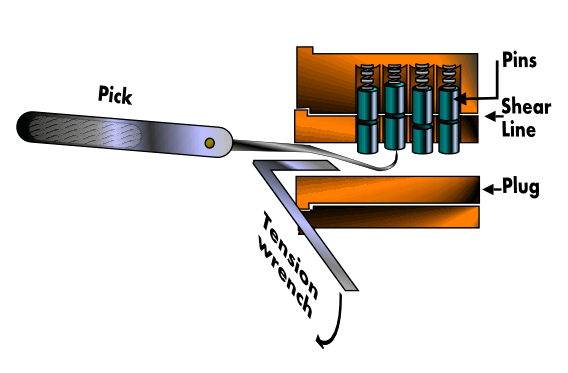
\includegraphics[scale=0.6]{./PinTumblerLock.png}
			\caption{Example of Picking a Pin and Tumbler Lock}
			\label{fig:PinTumblerLock}
		\end{figure}
		\subsection{How the Pin and Tumbler Lock Works}
			As can be seen in figure \ref{fig:PinTumblerLock}, this type of lock uses a number of sprint loaded pins which stop the plug of the lock moving within the housing. 
			Within this plug is a long, thin slot for the key (or our picks) with small ledges in the sides to both stop pins from falling and hinder those attempting to pick the lock. 
			A series of holes are drilled through the top of the housing and into the plug. 
			These holes are where the spring loaded pins enter, with the lower pin fully entering the plug and the upper pin being split across the sheer point. 
			It is this action which both allows the lock to remain closed when the key is not inserted and allows us to pick the lock. 
			When a torque is placed on the plug, some of these pins will begin to bind with the sheer point. 
			Using this, we can begin to pick the lock. 

		\subsection{Pin by Pin Picking}
			The first step when attempting to pick a lock is to place the tension wrench into the bottom of the lock and apply a slight pressure. 
			This pressure is designed to cause the top pins to catch on the sheer point of the plug, allowing some of the pins to bind. 
			Once this has occurred, a pick should be used to test each of the pins, determining how many there are and which ones have become bound to the sheer point. 

			The idea here is to place a small amount of pressure on the pins which bind to the sheer point in order of their binding. 
			This should leave the upper pin lodged above the plug, with the lower pin dropped into the keyway. 
			Continue with this until either you have bound all pins and the lock is open, or you cannot determine whether pins have set or not. 
			If the latter, reset the pins by releasing pressure on the tension wrench. 
		\subsection{Raking}
			If on the other hand, you are the kind of person with little patience and a strong desire to get in, you can attempt raking. 
			In this process, you set the lock up in the same manner, but rather than attempting to find and set binding pins, you simply saw along the line. 
			When attempting this, no more than two pins are likely to set on each pass, with passes that set no pins being common. 
			Thus, you should repeatedly attempt rake until either the lock opens or you feel that you are getting no where. 
			During this process, you may also want to slightly adjust the amount of torque placed on the plug, however, be wary not to place too much torque on it. 

	\section{Research}
\chapter{Network Operations}
	\label{ch:NetworkOperations}
	By using a common language and being able to write it down, the human race has been able to move from hunter gather to large scale society. 
	Language has allowed us to communicate the skills which our forebears learned to their children, eventually to us. 
	In a similar manner, computers need a means of communicating. 
	This is where networking and the OSI model for computer communications comes in, they allow computers to become more than just the machine in front of you. 
	Networking has become commonplace---many people would find no use in a computer without it---and many of our most used programs depend entirely on it. 
	However, to understand how to exploit networking, we need to understand how the communication takes place, how the network has been created and how to connect to the services running on other machines in ways they may not have been designed for. 
	\section{OSI Model}
		When computers are communicating, they need to be able to speak in the same language.\cite{HackingAOE} 
		However, if a programmer needed to implement this every time they required network communication, we would never achieve communication between two systems.\footnote{\url{https://xkcd.com/927/}} 
		Due to this, the OSI Model was created. 
		The OSI model provides the standards for all levels from the application currently being used to the bare metal the data is sent over. 
		These standards allow the relevant equipment to focus on the necessary parts of their implementation, while the other parts are taken care of, allowing for easier communication between unlinked programs. 
		The layers of the OSI Model are as follows:
		\begin{description}
			\item[Physical Layer]
				Deals with the physical connection between two machines through means such as CAT5 ethernet. 
				This is the lowest layer, whose primary role is communicating raw bits, as well as starting maintaining and ending the transmission. 
			\item[Link Layer]
				Transfers data between the two points connected by the physical layer. 
				This layer provides some high level functions which allow for error correction and flow control. 
				It also provides a means of activating, maintaining and ending the link. 
			\item[Network Layer]
				Provides a means of transmitting datagrams from one machine on the network to another. 
				This is the layer where network addresses (IP) are translated into a physical machine address. 
			\item[Transport Layer]
				Provides transparent transfer of data by allowing reliable communication and known protocols. 
				This layer means that higher layers need not worry about reliability of connection. 
			\item[Session Layer]
				Responsible for establishing and maintaining connections between applications. 
			\item[Presentation Layer]
				Presents the data to the application which is is being communicated to in a format which is understandable to the application. 
				This is the layer which allows for encryption and data compression. 
			\item[Application Layer] 
				Keeps track of the requirements of the application and allows it to utilize the data which it received. 
		\end{description}
		When data is transmitted through these layers, it is encapsulated in quanta known as packets. 
		Each of these packets contains the metadata required for each of the layers of the network model. 
		Starting from the application layer, each layer that the packet passes through will add a new header for it's data, which will not be read until the packet passes through that layer on the other end of it's journey. 
		%TODO: Think about using a figure here to show this encapsulation. 
		This layered nature allows us to connect using sockets, handling only the application and presentation layers and allowing the OS to sort the rest for us. 
	\section{Network Architecture}
	\section{Connecting to Networked Software}
	
\chapter{Network Penetration}
	\label{ch:NetworkPenetration}
	Network penetration is a multiphase process, starting at information gathering with tools such as nmap and Nessus, and moving on to gaining and maintaining a presence through exploitation. 
	This chapter will show a step by step progression through this, explaining how an attacker would find their target on a network, exploit it and move on to another target without losing control of the first machine. 
	\section{Nmap}
		Port scanning is a simple way to determine what services are running on a computer. 
		This can be done due to the fact that most programs run on a known port specified in their documentation. 
		However, it also works by fingerprinting the response, which is usually specific to the program which is running on the port. 
		This can be done through a number of means, such as attempting to open a full TCP connection to each port or only attempting a partial connection. 
		It must be noted that while effective, the former is rarely used due to the ease of detection and large amount of network traffic generated. 
		Nmap\cite{NmapBook} is the tool that we will utilise to conduct these scans. 
		It has a number of options which allow us to control the scan to our exact specifications and commonly picks up most services.\cite{HackingAOE} 
		\subsection{SYN Scanning}
			The most common scan used is known as a SYN scan. 
			This will send TCP SYN packets to the specified ports on the target computer, listening for the SYN/ACK response. 
			If a SYN/ACK packet is received, the port is marked as open, the packet is examined for service fingerprinting and an RST packet is sent to stop the connection and prevent accidental DoS. 
			Using nmap, the ``-sS'' flag is used to run a SYN scan. 
			\begin{quote}
				nmap -sS <Target IP>
			\end{quote}
			This will output all of the services which are found to be running on the remote system. 
			A sample output of an nmap SYN scan can be seen below. 
			Note that this is an exaggerated response, as the target scanned was intentionally vulnerable. 
			\begin{verbatim}
				Starting Nmap 7.01 (https://nmap.org ) at 2016-01-17 00:56 EST
				Nmap scan report for 192.168.115.129
				Host is up (0.000099s latency).
				Not shown: 977 closed ports
				PORT     STATE SERVICE
				21/tcp   open  ftp
				22/tcp   open  ssh
				23/tcp   open  telnet
				25/tcp   open  smtp
				53/tcp   open  domain
				80/tcp   open  http
				111/tcp  open  rpcbind
				139/tcp  open  netbios-ssn
				445/tcp  open  microsoft-ds
				512/tcp  open  exec
				513/tcp  open  login
				514/tcp  open  shell
				1099/tcp open  rmiregistry
				1524/tcp open  ingreslock
				2049/tcp open  nfs
				2121/tcp open  ccproxy-ftp
				3306/tcp open  mysql
				5432/tcp open  postgresql
				5900/tcp open  vnc
				6000/tcp open  X11
				6667/tcp open  irc
				8009/tcp open  ajp13
				8180/tcp open  unknown
				MAC Address: 00:0C:29:92:21:5E (VMware)
	
				Nmap done: 1 IP address (1 host up) scanned in 13.38 seconds
			\end{verbatim}
		\subsection{Other Scan Types}
			While SYN scanning is useful, it has become easier to detect due to the introduction of IPS with partial connection rules. 
			These systems will see a number of partial connections within a given time and will lock out the address that the connections came from, effectively halting your scan. 
			To combat this, a number of other scan types have been created, each exploiting some part of the network standard. 
			These newer scans work by sending a TCP packet which doesn't make sense to each port. 
			When these packets are received by a service, they will be ignored. 
			However, when the OS receives them on a closed port, it will often reply with a RST packet. 
			This difference can be used to determine which ports are open. 
			This will work on any system which follows the RFC793 standard. 
			Most *nix systems following this, however, windows does not. 
			\begin{description}
				\item[FIN scan]
					sends a FIN packet. 
					Used by specifying ``-sF'' in nmap. 
				\item[X-mas scan]
					sends a packet with FIN, URG and PUSH flags on.
					Used by specifying ``-sX'' in nmap. 
				\item[null scan]
					sends a packet with all flags off. 
					Used by specifying ``-sN'' in nmap. 
			\end{description}
			These scans will generally give you exactly the same output as the SYN scan, except where RST replies are not sent or where SYN scans are blocked by a firewall. 
			When you don't care about hiding and would like as much information as possible, all nmap scans can be integrated by using the ``-A'' option. 
			This will turn on all scanners, taking significantly more time and producing significantly network noise, however, you will receive detailed information on the services and OS running on the target. 

		\subsection{Other Means of Hiding}
			By default, many of these scans can be both loud and obvious to the trained eye or IDS.\footnote{\url{https://nmap.org/bennieston-tutorial/}} 
			Thus, nmap also comes with a set of flags which will enable you to attempt to hide the most obvious parts of the scan. 
			These, when used well will allow you to run an scan which will not be noticed by most of the IDS which are on the market today. 

			By default, nmap adjusts it's timings based on network speed and the response times of the target. 
			However, you are able to adjust these timings in order to either avoid detection or have the scan complete as quickly as possible. 
			These start with the ``-T0'' or paranoid scan, which will send packets at 5 minute intervals. 
			This timing will likely not be picked up by an IDS, nor by after the fact analysis due to the fact that random Internet traffic usually presents this number of invalid packets. 
			On the other end of the spectrum is the ``-T5''  or insane scan. 
			This scan will map a network exceptionally fast, but will trip most IDS systems and will be obvious in logs. 
			Furthermore, if you are on a slower network connection, it is possible that this scan will fail or drop data due to the high data rate required. 
			Further adjustment to specific parts of timings can be made, but this is usually not necessary. 
			See the nmap manual for more information on these. 

			If you are attempting to hide that you are the attacker, the decoy option ``-D'' will allow you to specify a number of IP addresses from which it will seem the attack originates.
			While this will not hide your own address, it will place it within a swath of other information, making it difficult to determine the original attacker. 
			Furthermore, when looking at logs, the target will assume that they were being scanned by a large number of hosts, causing them to worry about the potential future attacks. 

			For another level of stealth, ICMP pings can be turned off.
			These will make the scan less likely to be picked up in as the machines being scanned will not have a ping going out to test whether they are up first. 
			Furthermore, it will allow nmap to scan all hosts, rather than just those responding to ping. 
			When using this flag, you can also specify flags such as ``-PT'' or ``-PS'' which will send a TCP or SYN ping respectively. 
			There are a number of options for ping within nmap scans. See the ``-Px'' flags within the nmap manual. 

			A final option for bypassing firewalls is to use the fragment or ``-f'' option. 
			This will split every packet sent to the target into a number of small packets, which many firewalls will not attempt to reassemble before scanning them. 
			While this means that you are more likely to get past the firewall, it also can crash some less stable software and hardware. 
			Thus, this should be used with care, as crashing computer systems are exceptionally noisy. 
	\section{Nessus}
	\section{Metasploit}
	\section{Pivoting}
	\section{Maintaining a presence}
\chapter{Web Penetration}
	\label{ch:WebPenetration}
	\section{XSS}
	\section{SQL Injection}
	\section{File Uploads}
\chapter{Forensics}
	\label{ch:Forensics}
	\section{File Carving}
	\section{Steganography}
	\section{Wireshark}
	\section{Netflow}
\chapter{Reverse Engineering}
	\label{ch:ReverseEngineering}
	\section{x86 Assembly}
		%TODO: Decide whether this goes here or in programming. 
	\section{Radare2}
		Radare2 is a set of tools for working with binary files. 
		This makes it useful as a means of reading and altering compiled programs and their data files from the commandline. 
		While the Radare2 suite has a number of standalone programs within it, this section will cover only the main program. 
		This program allows for the searching, altering and disassembly of binary programs in multiple modes, making it a great tool for challenges such as Pwn Adventure in the next section.
		For a more detailed guide, read through the Radare2 book.\cite{Radare2}

		\subsection{Getting Started}
			The learning curve at the start of using Radare2 is quite steep. 
			However, if you have any experience with other commandline tools such as Vim and GDB, many of the commands and shortcuts should come easily. 
			Before going any further, it is worthwhile to note that you can get the help information for any command by appending a ``?'' to it. 

			Navigation within Radare2 is done through the following commands:
			\begin{description}
				\item[Seek]
					or ``s'' will move you to the address that you specify after the command. 
					The address can either be an explicit memory location, or a mathematical statement based on the current location or a label within the binary. 
					An example of this is ``s 0x00001c80''.
				\item[is]
					or information symbols will get you a list of the different symbols which are still in the binary. 
					These can be functions, objects, strings or any other symbol that survives the compilation process. 
					This is useful to find the functions which the program uses, and will become the main way of navigating in the Pwn Adventure Challenge. 
				\item[Visual mode]
					Like Vim, Radare2 has a visual mode which allows for direct reading and writing of assembly or hex. 
					In this mode, you can move using the same key bindings as Vim, with ``i'' being used as replace and ``p'' being used to change visual mode. 
					Furthermore, to get a cursor which can be used for these insert functions, use ``c''.
					This mode allows for the editing of the disassembled binary without having to reassemble it. 
				\item[Hex View]
					In visual hex view, hold shift while moving to highlight a byte range. 
					Tab will switch from the Hex pane to the ASCII pane. 
				\item[\~{}]
					This is the internal grep function. 
					When it is placed after a command, anything after it will be used to filter the results. 
					Furthermore, output can be filtered by column using the syntax ``[x]'' or by row using ``:x'' after the grep search.
			\end{description}
			Beyond this, you will want to start the program with the ``-w'' flag in order to write to the file. 
			Finally, any CLI program---or syntax such as pipes and redirection---installed on your computer can be accessed through the Radare2 prompt. 
			This is useful for actions such as greping through the output of ``is''. 

			At this point you should have enough of an understanding of Radare2 to be able to use it. 
			The next section contains spoilers to the challenges presented by Pwn Adventure 3. 
			Before reading on, recommend downloading and installing the game and attempting to reverse engineer it so that you can win. 
			I recommend starting with the sprint speed. 
			%TODO: Should there be more than this section here?
	\section{Pwn Adventure}
\chapter{Programming}
	\label{ch:Programming}
	\section{Introduction to the CLI}
		The commandline is the tool for direct interaction with your computer. 
		It is like the baby brother to programming yourself, though with scripting it can become just as complex. 
		The commandline will enable you to tell the computer what you want it to do, rather than stepping through a long list of clicks in order to have a program do what it thinks you mean. 
		This gives you fast and powerful interaction with your computer, but it is not without a steep learning curve. 
		This section will focus on the \**nix bash shell, which is the most common powerful shell used today. 
		Others such as powershell on windows and Zsh on \**nix are not to be discounted, but bash will get you the furthest with minimal training.\cite{CLICrashCourse}
		What follows is a basic introduction to the most common commands, an easy way to remember what they do and their usage:
		\begin{description}
			\item[pwd]
				Where am I?
				Whenever you are lost, this will show you where you are in the filesystem. 
				It is similar to the URL bar in a browser or file manager. 
			\item[hostname]
				What machine am I on?
				This will allow you to determine what machine your current session is running on. 
				It can be useful when you think you have opened a shell to another computer but aren't sure. 
			\item[mkdir]
				Like selecting new folder, but four steps in one. 
				Run it as ``mkdir <folder name>'' to create one folder or run it with the ``-p'' argument to create a whole branch of directories, separate each folder name with ``/''. 
			\item[ls]
				List the contents of a directory.
				This will give you the contents of the directory you are in, or the one you have given as an argument. 
				The following are useful flags for ls:
				\begin{itemize}
					\item -l long, gives you sizes, permissions change times and other information. 
					\item -h gives you data in a human readable formate. 
					\item -a all, gives you all files, including hidden files (also known as dotfiles)
					\item -S sort size, gives you all files in the directory sorted by size. 
				\end{itemize}
			\item[cd]
				Tell the computer where you want to go. 
				cd will take you to the location within the filesystem that you give as an argument. 
				Furthermore, it takes advantage of special characters within \**nix systems such as ``.'' and ``..'' which mean current and previous directory along the current branch of the filesystem. 
			\item[rm]
				I want this file gone. I want it burned. 
				When using this command, you will lose the file, either understand the wildcards you are using, or get good at file recovery. 
				Alone, this command will delete files, using the ``-r'' flag will allow it to recurse through directories. 
				Furthermore, some systems have added the flag ``--no-preserve-root'', which will stop you deleting your entire system. However, the existence of this flag should not be trusted. 
				For example, it does not exist on Mac OS X. 
			\item[touch]
				Create a file here, I don't care about type or content. 
			\item[cp]
				Copy and paste. Used as ``cp src dest''.
			\item[mv]
				Cut and paste. Used exactly the same as cp. 
			\item[less]
				Read a file which would cause your terminal to scroll. 
				Use page up and down or the arrow keys to navigate. 
				Use ``/'' to search.
				Quit by pressing q.
			\item[cat]
				Stream a file to your STDOUT. 
				This can be useful for small files, checking that a change occurred properly or piping a file into another command. 
				It is little known, but this command stands for concatenate. 
				Thus it can be used to merge a number of small files into a large one using ``cat file1 file2 file3 > bigFile''.
			\item[Pipes]
				The pipe, ``|'' is used to send the output of one command to another. 
				This would be useful for example to edit a file by streaming it from cat into sed. 
			\item[Output Redirecton]
				This is useful to force a program to read or write to or from a file. 
				It works in the following manner:
				\begin{itemize}
					\item ``> <outfile>'' Write output to a given file.
					\item ``< <infile>'' Read the given file as input.
					\item ``>> <outfile>'' Append the programs output to the given file. 
						%TODO: Fix the rendering of the >>
				\end{itemize}
			\item[\** wildcard]
				This is the most simple wildcard. 
				It is used to match anything which follows the form given to it. 
				For example the command ``cat /etc/\**.conf'' would print to STDOUT every ``.conf'' file in ``/etc''.
			\item[locate]
				Database search for the whole filesystem. 
				If you need it, and it exists, locate knows where it is. 
				However, you may need to run updatedb first. 
				Use this command as ``locate <pattern to search for>''
			\item[find]
				When locate is not installed (such as with most Mac OS X installs) find will do the same job. 
				However, find has to run through the filesystem each time the command is run, making it far slower for large searches. 
				This command works the same as locate. 
			\item[grep]
				Search for a given pattern within a pipe or stream. 
				This will also work for redirects and can be used on an individual file. 
				Used as ``grep pattern'', and can use flags such as ``-i'' to ignore case. 
			\item[man\footnote{\url{http://linux.die.net/man/}}]
				When you're inevitably told to RTFM, this is where you go. 
				Used as ``man <command>'', this program will give you the manual entry for the given command, spelling out all of the flags and usages which you may want. 
				An alternative to this is using ``<command> \verb+--+help'' or ``<command> -h'' which may show a shortened version. 
			\item[dd]
				A low level copy of the given partition or disk. 
				This command ignores filesystem and just writes the bits read from the input device to the output. 
				It is used as ``dd if=<input file> of=<output file>''.
				Be wary that if this command is entered wrong, you will loose data. 
				It can also be combined with other commands, such as ``dd if=<in> | pv -s <size>G | dd of=<out>''.
			\item[vim]
				The editor war will likely never end, and each side will tell you to use their preferred. 
				Vim is a powerful editor which I am using to write this. 
				However, it can have a steep learning curve, and thus must have time dedicated to it's usage. 
				Following the tutorial provided by the command ``vimtutor'' will give you the basics that you need to begin using vim properly. 
				However, if you do not wish to learn a fully featured editor, the likes of ``nano'' and ``ed'' will serve you well. 
		\end{description}
		While there are many other commands\footnote{\url{https://github.com/jlevy/the-art-of-command-line}} commonly installed with a \**nix system, these are the most common and some of the most useful. If you would like to learn more, the footnotes throughout this section have detailed information on many more commands. 

	\section{Introduction to Powershell}
	\section{Introduction to Scripting}
	\section{Introduction to Python}
	\section{Introduction to C}
	\section{Programming Challenges}
\chapter{Cryptography}
	\label{ch:Cryptography}
	\section{Introduction to Cryptography}
	\section{Utilizing Cryptography in Python}
	\section{Poor Cryptography Implementations}
	\section{Hash Cracking}
		Hashes are used in many situations to store passwords. 
		This is done because the hashing algorithm is a one way action, meaning that there is no easy way to calculate the password from the hash. 
		Due to this, the means of authentication on most programs is done by hashing the entered password and comparing it to a stored hash. 
		If the two match, it is likely---though not guaranteed due to collisions---that the password is the same. 
		While this may sound like it makes attacking these targets hard, it is far from being unsolvable. 
		Tools such as ``John the Ripper'' and ``Hashcat'' can be used to compute hundreds of thousands of hashes per second, which can then be compared with the given hash. 
		This makes hash cracking a matter of time and dictionary crafting. 
		\subsection{John the Ripper}
			While there are many tutorials\footnote{\url{http://openwall.info/wiki/john/tutorials}} on the usage of John the Ripper(John) which go into specific detail, this section will explain the basic usage of the tool. 
			Before starting, check that the version of John which you have installed is correctly compiled for your system, you may want to enable options such as gpu cracking, which needs to be done at compile time. 
			What follows is a list of common commands for use with John:
			\begin{description}
				\item[-single]
					The simplest means of attacking a hash. 
					This mode uses only a basic wordlist and very few rules. 
					Thus it is not recommended for anything but the most basic attacks. 
				\item[-wordfile:]
					Uses the wordlist specified directly after the colon. 
				\item[-rules:]
					Specifies the mutation rules for the given wordlist. 
					These can be used to create a dictionary with substitutions, such as 1337 speak. 
				\item[-incremental:]
					This, along with options such as ``alpha'', ``digits'' or ``lanman'' will give you a brute force of letters, numbers or both with some special characters respectively. 
				\item[-external:]
					Allows the use of pre-configured modes, which can be powerful if used or modified correctly. 
					%TODO: add more to this and rules. 
				\item[-restore:]
					Will start a crack part way through based on a restore file created by a previous session. 
				\item[-sesion:]
					Used to name the restore file that will be created when the session is broken. 
				\item[-status:]
					Shows how far into the crack a previous session was stopped. 
				\item[-show]
					Shows how many passwords within a file have been cracked and how many remain. 
				\item[-format:]
					Specify the hash format (such as SHA512) which the hash to crack was created with. 
			\end{description}
			
		\subsection{Hashcat}
			Hashcat was started due to the fact that at the time, tools such as John the Ripper did not make proper use of multithreading. 
			This has been expanded to include GPGPU processing using tools such as openCL and CUDA, and has made hashcat one of the fastest hash cracking tools currently available. 
			Both Hashcat and the newer oclHashcat use the same input files and command syntax. 
			However, oclHashcat will conduct the crack on the GPU installed on the system, rather than the slower CPU. 

			Hashcat uses a number of modes to allow it to crack hashes. 
			Each of these modes has a number of specific properties which make it better at a given type of attack. 

			\subsubsection{Mask Attack}
				This attack, while similar to a brute force attack, uses a mask to reduce the possible character set of the attacks.\footnote{\url{http://hashcat.net/wiki/doku.php?id=mask_attack}} 
				Rather than run through every possible permutation of the character space for every character in the password, the mask attack requires that the user input some details of the characters within the password. 
				
				When using this mode, for each position within the password, we need to create a mask using either the character sets outlined in table \ref{tab:HashcatMaskCharSets} or a custom character set defined before starting. 
				\begin{table}[htb]
					\centering
					\begin{tabular}{| l | l |}
						\hline
						?l & abcdefghijklmnopqrstuvwxyz \\ \hline
						?u & ABCDEFGHIJKLMNOPQRSTUVWXYZ \\ \hline
						?d & 0123456789 \\ \hline
						%?s & \verb¤«space»!"#$%&'()*+,-./:;<=>?@[\]^_`{|}~}¤ \\ \hline
						?s & Special Characters \\ \hline %TODO: Have this print the characters. 
						?a & ?l?u?d?s \\ \hline
						?b & 0x00 - 0xff \\ \hline
					\end{tabular}
					\caption{Hashcat Mask Mode Built in Character Sets}
					\label{tab:HashcatMaskCharSets}
				\end{table}
				Attacks in this mode are limited by the length of the mask given. 
				This means that if you give a mask with 8 character spaces, but have a password which is 6 characters long, you will be unable to crack it. 
				Due to this, the ``\verb+--+increment'' flag was created. 
				Furthermore, a list of standard character sets for multiple languages can be found in ``/usr/share/hashcat/charsets/''.

				Another means of creating this attack mode is to use a Hashcat Mask File. 
				These files contain a number of masks and the custom character sets which are used within them, in order to run attacks which are regularly repeated. 
				To use one of these files, run Hash cat with the arguments ``-a 3 <hash file> <mask file>''.

			\subsubsection{Dictionary Attack}
				In this attack, a dictionary or word list is created to be utilised within the attack. 
				This dictionary can either be one that you found on the system or one that was created specifically for the job. 
				Due to the limitations of this attack, it is recommended that it is either used with a specifically generated dictionary, which can be done by a program such as John the Ripper or
				a can be manually written through the use of a python script. 
				This type of attack may be the first that you use, as it will likely be the quickest attack. 
			\subsubsection{Combinator Attack}
				In this attack, each word of a dictionary is appended to each word in a second dictionary. 
				This will catch many passwords which use two simple words, as long as the dictionary is well written. 
				However, if the dictionaries that you are using have already been enumerated in such a way, it will likely not produce useful results. 
				Furthermore, this attack will not run the words from each dictionary separately. 
				To use this attack, run the top command for GPU or the bottom command for CPU. 
				\begin{quote}
					oclHashcat64 -m 0 -a 1 <hash file> <dict1> <dict2>
					
					hashcat-cli64 -m 0 -a 1 <hash file> <dict 1 and 2>
				\end{quote}
			\subsubsection{Hybird Attack}
				This attack uses the concepts of both the combinator and mask attacks. 
				This means that you can specify a dictionary and have hashcat add the mask that you give to either the start or end of the word. 
				Using this means, you can easily run through passwords such as name and birth year combinations. 
				To conduct this attack, use the command:
				\begin{quote}
					oclhashcat -a 7 <mask> <dict>
					\\or\\
					octhashcat -a 7 <dict> <mask>
				\end{quote}
				
		\subsection{Rainbow Tables}
			In both of the previous sections, we have been calculating the hashes which we are testing against the password hash on the go. 
			This means that we have to calculate the algorithm, sometimes multiple thousands of times, for each password we want to try. 
			There is another option: rainbow tables. 
			This method of cracking passwords allows us to have a precomputed list of hashes and their respective passwords, which we then simply search through. 
			This results in two significant differences:
			\begin{itemize}
				\item Password cracking takes seconds
				\item Your hard drive is full. 
			\end{itemize}
			However, these tables are not the be all and end all of hash cracking. 
			They rely on the hashes being computed either with no salt or with the same salt as the table, meaning that hashes generated using a randomized salt will not be vulnerable. 
			Furthermore, they rely on the attacker being able to find a table which will suit the password. 
			Thus, if your password is a 50 character essay with special characters, it will likely not show up in the table due to size constraints. 
			Such a table would have to contain $\approx2.49\times10^{66}$ password--hash pairs, resulting in a file size of $\approx2.6\times10^{44}$Yottabytes.
			Though this cannot be thought of as a limitation when compared to the two other methods, as for the same password, they would take $\approx5.2\times10^{52}$ years on 3 ATI HD7970 GPUs.\footnote{\url{https://litecoin.info/Mining\_Hardware\_Comparison}}
			At this point, even assuming Moore's law continues and Processing power becomes far cheaper, the password will not be cracked within a reasonable time frame. 

			It is for these reasons that rainbow tables are uncommonly used outside of cracking hashes from poorly implemented software with short passwords. 
			However, if you know that the character space is small, and either the passwords are unsalted or the salt is commonly known, rainbow tables are the best method if you have the storage space. 
		\subsection{Online Methods}
			With the rise of cloud computing and cheap server rental, many people have begun using tools such as Amazon Web Services to run crack servers. 
			This is done by deploying the tools shown above into a server which has been rented with multiple GPUs. 
			This server can then be optimised such that the cracking will properly utilise the GPUs of the machine as well as only calculating hashes that have a possibility of being correct. 
			Thus, as above, if you know that the hash will be within a given dictionary, or that it does not contain special characters, use these functions. 

			While this will work, and usually faster than using one's own computer, it is not as fast as a dedicated cracking cluster. 
			These clusters work by having a number of machines, each with the necessary hardware and software installed working together on the one hash. 
			Programs such as Hashcat can be used to control up to 125 GPUs across the cluster in order to crack the hashes you provide. 
			This method, while expensive and difficult to set up, is currently the fastest means of cracking a hash. 
			However, if you set your cracking program up properly, it will still likely beat this setup when it is brute forcing hashes. 
		\subsection{Salting}
			Many of the methods above become significantly more difficult when salting is introduced. 
			Normally, a hash will be produced by simply running a hash function on the password ($hash(pass)$). 
			However, when salting is implemented, the hash may be generated by adding either a known string or a random string---or sometimes both---to the password before passing it to the hash function ($hash(pass + "salt"$ or $hash(pass + rand()$).
			In either of these cases, the salt must be stored, which has led to split salting, using a random stored value or the users name/ID as well as a hard coded element. 
			This makes knowing the salt hard, but not impossible, as we can reverse engineer the code in order to determine the salting algorithm used and a simple ``strings'' on the compiled code will give us a hard coded salt string. 
			Nonetheless, these methods deter attackers from attempting to crack the hashes by limiting their choices and removing their ability to use rainbow tables. 
	\section{Challenges}
		\subsection{Hash Challenges}
			This first challenge is based on the \href{https://xkcd.com/936/}{xkcd comic ``Password Strength''.}
			The wordlist for this challenge can be found by using the following command on kali linux:
			\begin{quote}
				head -n 20 /usr/share/wordlists/rockyou.txt
			\end{quote}
			The password, hashed in MD5 and SHA256 can be found below. 
			\begin{verbatim}
				MD5: 
				4aa6dea37dec500f58bb241404471981
				SMA256: 
				6ff13e15281e9953d2c85c86e3727ea1cf3862f44d5cf18961811d63eebce2da 
			\end{verbatim}
			While you can complete this in any way you like, I recommend either using John's rules, or creating a custom wordlist and using Hashcat's hybird mode. 
			%Solution: "N1c0l3;7"

			The second challenge is based on an ATM keypad. 
			Through an image captured when the hash was pulled, it was determined that the only keys pressed were ``2, 4, 9 and 0''. 
			The password was also determined to be exactly 16 characters long. 
			Create a custom mask for Hashcat and solve this sha256 hash. 
			\begin{verbatim}
				27e4c844657fee60da199ccb1b60c0f4072370633b1a6e831141dbf9ab4e6b01
			\end{verbatim}
			%solution: "2490092442902942"

			The third challenge is based on using multiple dictionary words. 
			This is a common method used to create passwords. 
			I recommending using Hashcat in combinator mode to solve this SHA256 hash. 
			All the words necessary to solve this can be found in the rockyou wordlist. 
			\begin{verbatim}
				2fb26990a2b7d9ba876668c0ed6c9e9006313286ae02e7224e18939833fb9096
			\end{verbatim}
\chapter{System Hardening}
	\label{ch:SystemHardening}
	Securing one's own operating system and the software within can be a daunting task. 
	One must way up the needs of security against the usability of the system, or face months of instability or system management on a broken system. 
	Thus, for each recommendation below, decide how the computer needs to work for you and implement it to that level.\\ 
	If the newly secured system does not work for you, simply roll it back until it does. 
	When implementing this, remember that the biggest threat will always be the user of the system. 
	Thus, security must be implemented in layers, each of which is able to stop attacks which may have breached the outer layers. However, no matter how secure the system is made, if it is on, it is vulnerable. 
	Each section within this will be referenced in the footnotes. See those references for information on the implementation of these notions. 
	\section{Linux Hardening}
		Due to the varied nature of Linux distributions, it is difficult to provide an exact guide to securing an arbitrary Linux install. 
		However, this section will discuss the protections which will work on the general system.\footnote{\url{http://www.asd.gov.au/publications/protect/top\_4\_mitigations\_linux.htm}} 
		For distribution specific guides, look to your distribution's guides\cite{FedoraSecGuide}or wiki.\footnote{\url{https://wiki.archlinux.org/index.php/Security}}
		\subsection{Passwords} 
			Your password are the key to having a secure system. 
			Especially once disk encryption and password managers are in use, they can be the downfall of one's entire computing presence. 
			Thus, passwords should be created and managed in a secure way:
			\begin{itemize}
				\item Not containing personal information.
				\item Not dictionary words or common substitutions (such as 1337Speak)
				\item Not having all numbers or symbols at the start or end. 
				\item Not a common short phrase. 
				\item Using an uncommon or nonsensical phrase such as ``Correct horse battery staple''\footnote{\url{https://xkcd.com/936/}}
				\item using multiple numbers, letters and symbols. 
				\item Randomly generated using a password manager. %TODO: \ref this to browser hardening PMs 
				\item Longer than 12 characters. 
			\end{itemize}
		\subsection{Password Hashing}
			Linux stores hashed passwords in ``/etc/shadow''. 
			It is worthwhile checking the settings of your Linux install to ensure that passwords are hashed properly and with a number of rounds. Thus, open ``/etc/pam.d/passwd'' and ensure that it contains the line:
			\begin{quote}
				password required pam\_unix.so $\textbf{sha512}$ shadow $\textbf{rounds=65536}$
			\end{quote}
		\subsection{Disk Encryption}
			is the process of automatically cryptographically protecting a part or all of a storage device.
			\footnote{\url{https://wiki.archlinux.org/index.php/Disk\_encryption}}
			When properly utilized, disk encryption will ensure that only a trusted user will be able to unlock the computer. 
			However, the system will still be vulnerable to remote attacks, cold boot attacks and coercion (though this can be mitigated through plausible deniability)
			The following is a description of the types of encryption and their effects on security"
			\begin{description}
				\item[Data Encryption] Encrypting nothing more than the data. 
					This is useful for privacy concerns and is the easiest to implement. 
					However, date encryption will not protect from OS tampering such as installing keyloggers as well as cache attacks, taking advantage of data cached in locations such as ``/tmp''.
				\item[System Encryption] Encrypting the whole OS and all user data. 
					This prevents the two downfalls of data encryption by ensuring that any tampering will cause a garbled output on the OS disk and that call caches are encrypted. 
					However, this requires that the boot system be aware of the encryption and that a password is entered before boot. 
			\end{description}
			In order to achieve this, there are two types of encryption which may be utilized:
			\begin{description}
				\item[Stacked Filesystem Encryption] A designated folder within the filesystem which encrypts files before they are written to the disk. 
					This means that the files will be visible from the encrypted filesystem, but the names and data will be encrypted until unlocked. 
					This is a simple means of Data Encryption. 
				\item[Block Device Encryption] Operates below the filesystem, encrypting the filesystem and the files contained within it. 
					In this type of encryption, the contents of the whole device will look like random data rather than a filesystem filled with random files. 
			\end{description}
		\subsection{Mount options}
			When setting up a secure environment, one should take care to give the least permission required to conduct a task. 
			Thus, when mounting file systems, it is best to limit what can be done with the data on the system.
			There are three restrictions which can be placed on a mounted filesystem:
			\begin{description}
				\item[nodev] Do not interpret character or block special devices on the filesystem
				\item[nosuid] Do not allow set-user-identifier or set-group-identifier bits to take effect
				\item[noexec] Do not allow execution of binaries or other files found in the filesystem. 
			\end{description}
			A basic guide for what common filesystems can be mounted with which options can be found in table \ref{tab:mountOptions}, use these within the file ``/etc/fstab''.
			\begin{table}[htb]
				\centering
				\begin{tabular}{| l | l | l | l |}
					\hline
					$\textbf{Partition}$ & $\textbf{nodev}$ & $\textbf{nosuid}$ & $\textbf{noexec}$ \\ \hline
					/var  &		yes &	yes &	yes \\ \hline
					/home &		yes &	yes &	if you do not code or use wine \\ \hline
					/dev/shm &	yes &	yes &	yes \\ \hline
					/tmp &		yes &	yes &	breaks compiling packages \\ \hline
					/boot &		yes &	yes &	yes \\ \hline
				\end{tabular}
				\caption{Common filesystem restrictions}
				\label{tab:mountOptions}
			\end{table}
			\subsection{File Permissions}
				The default file permissions allow almost all files to be read by all users, while writing and executing is reserved for the owner and root. 
				This means that if any user is compromised, most files on the system can be stolen. 
				Furthermore, it means that the attacker can use the systems configuration files to determine likely privilege escalation or pivot points. 
				To solve this, important configuration files permissions should be set to 700 and the default umask should be set to 077. 
				This will ensure that only root can read and change configuration files and only root and the owner can read their own files. 
				This is especially important in a multi-user system, where other users would otherwise be able to read all users data. 
			\subsection{Users}
				One of the first things to do on a new Linux install is to create a new user to use rather than root. 
				This removes a large point of failure in that if the root account is compromised, the whole system is.\\ 
				To add to this, one should look to implement lockouts on failed login attempts through the pam\_tally\footnote{\url{http://linux.die.net/man/8/pam\_tally}} system.
				This system will ensure that if a user attempts to access the system with an incorrect password, they will be locked out, either for a given time, or until unlocked by the root user. 
				This avoids an opportunistic malicious user attempting to guess the password. \\
				Another means of securing users is to limit the number of processes which can be spawned by an individual user. 
				This will limit the effect of a user account being used to run a denial of service (DoS) attack on the system. 
				Furthermore, it will disallow actions such as fork bombs from bringing the whole system down. 
				This can usually be achieved by adding the following lines to ``/etc/security/limits.conf''
				\begin{quote}
					\begin{flushleft}
						\** soft nproc 100 \\
						\** hard nproc 200 \\
					\end{flushleft}
				\end{quote}
				
				In addition to this, services which are particularly vulnerable
				---such as any Internet facing services---
				should be run from an additional restricted user account. 
				This will ensure that if these services are targeted, it is more difficult to escalate to a privilege or root account. 
				Furthermore, by implementing this alongside the other recommendations specified here, 
				it becomes difficult for an attacker to take data, due to the fact that they cannot see most of the filesystem.

			\subsection{Restricting use of root}
				\begin{itemize}
					\item The sudo command should be used rather than su due to the following reasons:
						\begin{itemize}
							\item It logs commands and the users which invoked them
							\item Root password is held secure. 
							\item Prevents accidental execution. 
							\item Individual commands may be enabled for users or group through the sudoers file. 
						\end{itemize}
					\item sudoedit or sudo -e should be used rather than running an editor as root. 
						To do this, add ``SUDO\_EDITOR=<editor>'' to your environmental variables.
					\item Restrict root login both locally and via SSH. 
				\end{itemize}
			\subsection{Mandatory Access Control}
				MAC, as opposed to the Discretionary Access Control (DAC) used on most Linux systems is a rule set which designates which actions can be taken on which files and directories. 
				This rule set is created by the root user and unlike DAC cannot be altered by the users of the system. 
				While any MAC system will be far better than DAC, one must ensure that MAC is properly setup, as malicious execution during the learning phase could create vulnerabilities which will go undetected. 
				Furthermore, on the desktop, due to the wide variety of tasks which are completed, a poorly setup MAC will either be far too permissive or far too restrictive. 
				%TODO: Think about writing out the types here. Think about linking the implementations. 
				MAC can also be utilised as a means of creating application white listing.
				While difficult to create a strong policy, it is one of the best methods for running application white listing on Linux, 
				due to the fact that there is no prebuilt white listing tool. 
			\subsection{Kernel Hardening}
				The following are the common steps used to harden the Linux Kernel. 
				\begin{description}
					\item[Restricting access to kernel logs]
						These logs contain information which may be useful to an attacker, such as the software currently running and sensitive memory addresses. 
						To restrict access to these logs, add the line ``kernel.kptr\_restrict = 1'' to the file ``/etc/sysctl.d/50-kptr-restrict.conf''
					\item[Hidepid] 
						The kernel will hide the pid of processes owned by other users if this is enabled. This is done by mounting the ``/proc'' filesystem with the option ``hidepid=1''. 
					\item[Grsecurity\footnote{\url{https://en.wikibooks.org/wiki/Grsecurity}}]
						is a kernel which has been patched with multiple security enhancements. 
						Both the kernel and userspace are hardened against common memory corruption vulnerabilities along with the addition of PAX integration and a role based MAC system. This is the easiest way to secure the kernel itself against exploitation. 
				\end{description}
				\subsection{Sandboxing with firejail}
					Sandboxing is an important part of running a secure system. 
					It allows the user to run a program knowing that only specified changes (or none at all) will be made to disk. 
					Firejail\footnote{\url{https://firejail.wordpress.com/documentation-2/}} gives an easy way to do this through it's commandline interface. 
					The command ``firejail <program>'' will execute ``program'' in a sandbox. 
					For greater security, the command ``firejail \verb+--+seccomp \verb+--+private <program>'' will block ``program'' from writing anything to disk, effectively blocking all permanent changes. 
					While this latter case does not mean that the program cannot be used as a means to attack the machine, it does make it far more difficult. 
				\subsection{Firewall} %TODO: Add firewall chapter
				\subsection{Physical security}
					Given enough time and resources, physical access is root access. 
					However, a high level of security for both the operating system and data can be obtained through the use of a number of layers such as boot security and encryption. 
					It must be noted that the system can be tampered with by other means such as malicious hardware which can read and alter the memory of the computer while it runs. While there is little that can be done to avoid this outside checking for new hardware, it is unlikely that an attacker will be this knowledgeable or determined. 
					\begin{itemize}
						\item Implement a BIOS/UEFI password. 
							Though these are not completely secure, they ensure that the opportunistic attacker will be unable to alter the boot devices of the computer, forcing them to use your secured OS. 
							However, these can be worked around on most systems by wiping the CMOS. 
						\item Bootloader security should be implemented by either disabling editing of boot devices or adding a password to the bootloader. 
							This will stop the ``init=/bin/sh'' attack amongst others. 
						\item Deny root login from the console. 
							This would mean that the attacker would need both a username and password to access the system. 
						\item Set an automatic logout or use the lock features of the DE/WM that you use. 
					\end{itemize}
	\section{OS X Hardening}
		Hardening an OS X install\footnote{\url{https://github.com/drduh/OS-X-Security-and-Privacy-Guide}}, while similar in concept to Linux, is different due to the configuration system used by OS X. 
		Since it was derived from NeXTSTEP, it's configuration is written into binary plist files, which must be edited. 
		This guide will use the provided ``defaults'' program to edit specific parts of these files. 
		However, if you would like to edit them manually or learn more about the structure of these files, I recommend a text editor such as ``TextWrangler'' which can convert these files to and from binary. 

		\subsection{Full Disk Encryption}
			The built in FileVault utility makes full disk encryption on OS X easy. 
			This means that unless you need to access your hard drive from another computer for a good reason, FileVault should be enabled. 
			Furthermore, with more recent systems, FileVault will encrypt in hardware, ensuring that minimal performance losses are noticed. 
			As the initial encryption is based on the OS X PRNG, it is recommended that you use your system for a little while before enabling FileVault. 

			To enable FileVault, open the ``Security and Privacy'' settings and select enable. 
			This will then ask you to set a password, which will be used to encrypt your files.\footnote{\url{https://eprint.iacr.org/2012/374.pdf}} 
			Furthermore, it will generate a recovery key, which you should store in a secure place, as it is your only means of recovering data if you lose your password. 
			FileVault will offer to store this key with Apple, if you do this, you are removing any security you achieve by encrypting in the first place, so decline this offer. 
			At this point, you should alter some of the default key storage behaviours of OS X such as erasing the key from memory on sleep an enforcing hibernation. 
			This will mean that you do not have to manually turn off the computer for the encryption to be secure---the system need only be hibernating. 
			To do this, use the following commands:
			\begin{quote}
				sudo pmset -a destroyfvkeyonstandby 1
				sudo pmset -a hibernatemode 25
			\end{quote}
		\subsection{Firmware password}
			Unlike windows and Linux systems where the UEFI or BIOS are transparent to the user, Apple Mac computers attempt to hide this utility. 
			While it is not easy to access to the unaware, this is no means of security. 
			Thus, it is recommended that a password be placed on this utility. 
			This can be done through the following steps:
			\begin{enumerate}
				\item Holding the keys \keys{cmd + R} on boot to enter OS X Recovery mode.
				\item Choose ``Firmware Password Utility''
				\item Choose `` Turn On Firmware Password''
				\item Enter your password and quit the utility. 
				\item Hold the \Alt{} key during the next boot.
			\end{enumerate}
		\subsection{Firewall}
			The default OS X firewall is a good start for a blocking firewall. 
			However, it will not allow you to monitor connections, nor block outgoing connections.
			To enable it, use the command:
			\begin{quote}
				sudo defaults write /Library/Preferences/com.apple.alf globalstate -bool true
			\end{quote}
			To enable logging of blocked connections:
			\begin{quote}
				sudo defaults write /Library/Preferences/com.apple.alf loggingenabled -bool true
			\end{quote}
			To drop ICMP ping requests and TCP/UDP traffic on closed ports:
			\begin{quote}
				sudo defaults write /Library/Preferences/com.apple.alf stealthenabled -bool true
			\end{quote}
			See chapter \ref{ch:NetworkPenetration} for why this would be a good idea. 

			Finally, to prompt you for every application which attempts to receive an incoming connection, rather than allowing signed applications to receive this by default, run:
			\begin{quote}
				sudo defaults write /Library/Preferences/com.apple.alf allowsignedenabled -bool false
			\end{quote}

			At this point, you may wish to overcome the inability of the standard firewall for monitoring and outbound connections. 
			This can be done through either third party firewalls or the kernel firewall, ``pfctl''. 
			While I recommend the latter as it is built in, I recommend that you do more reading before enabling it. 

			\subsection{Services}
				OS X comes with a number of services which most people will not use. 
				Furthermore, many of these services phone home to apple or another organisation, either for monitoring or content purposes. 
				Use the following commands to gather information\footnote{\url{http://cirrusj.github.io/Yosemite-Stop-Launch/}} about the services currently running on your system:
				\begin{description}
					\item[launchctl list]
						view running user agents. 
						These programs were started by your user and are running in the background. 
					\item[sudo launchctl list]
						as above, but includes running system daemons.
					\item[launchctl list <Agent Name>]
						examine an agent or daemon.
					\item[defaults read <Agent.plist>]
						examine the job called by the agent. 
				\end{description}
				After using these tools, use tools such as the Unix manual and a web search to determine what the services do. 
				When reading a ``.plist'' file, look for ``Program'' or ``ProgramArguments'' to determine what the file runs, then search for the program. 
				To disable a service, use the following command:
				\begin{quote}
					sudo launchctl unload -w /System/Library/LaunchDaemons/com.apple.apsd.plist
				\end{quote}
				Noting that removing the wrong service will leave you unable to boot, requiring that you enable it again in single user mode.
				To check which services have been disabled, run the following command:
				\begin{quote}
					find /var/db/com.apple.xpc.launchd/ -type f -print -exec defaults read {} \textbackslash; 2>/dev/null
				\end{quote}
			\subsection{Spotlight}
				Spotlight is an exceptionally useful tool. 
				It is by far the quickest way to get information and launch programs on an OS X system. 
				However, in order to do this, is will often send data to both Apple and Microsoft. 
				To disable this, open Spotlight Preferences and uncheck ``Bing Web Searches'' and ``Allow Spotlight Suggestions in Spotlight and Look up''. 
				You may also need to disable this in Safari Preferences under ``Search''. 
				This will stop Spotlight from phoning home on every search. 
			\subsection{Homebrew}
				Many of the userland tools installed with OS X or the xcode package are vastly out of date BSD versions. 
				This can be resolved through the use of the Homebrew package manager. 
				This package manager uses TLS to pull down install scripts from it's git hub repository on Github.com, meaning that it is mostly secure so long as you trust the repository. 
				Nonetheless, it is recommended that you read through these scripts before running them, otherwise it is no different to running any arbitrary code on your system. 
				See the \href{https://github.com/Homebrew/homebrew}{Homebrew Github repository} for more information and installation instructions. 
				This will be used in further parts of this guide.
			\subsection{DNS}
				DNS leaks are the most common way for a computer to leak the locations they are accessing. 
				There are two steps to securing DNS requests, caching and encryption, both of which will be covered in this section. 

				Caching can be done with the dnsmasq program, which will store the results of requests rather than forcing you to request the address on every boot. 
				Furthermore, this program hooks into dnscrypt to encrypt your DNS traffic. 
				To install and configure both of these programs, run the following Homebrew script and commands:
				\begin{quote}
					brew install dnsmasq \verb+--+with-dnssec \\
					mkdir -p /usr/local/etc \\
					cp /usr/local/opt/dnsmasq/dnsmasq.conf.example /usr/local/etc/dnsmasq.conf \\ %TODO: This gets hyphenated. 
				\end{quote}
				At this point, you should configure both dnsmasq and dnssec to your preferences.\footnote{\url{https://wiki.gentoo.org/wiki/Dnsmasq}}	
				The configuration file is well commented, read through this as it should tell you what you need to enable. 

				Once configured, the following commands will properly install and launch the program. 
				\begin{quote}
					sudo cp -fv /usr/local/opt/dnsmasq/*.plist /Library/LaunchDaemons \\
					sudo chown root /Library/LaunchDaemons/homebrew.mxcl.dnsmasq.plist \\
					sudo launchctl load /Library/LaunchDaemons/homebrew.mxcl.dnsmasq.plist \\
				\end{quote}
				Then enable the local DNS server in the preferences for your network and any VPN that you are using. 

				In order to encrypt this traffic, you will now need to install dnscrypt. 
				\begin{quote}
					brew install dnscrypt-proxy \\
					sudo cp -fv /usr/local/opt/dnscrypt-proxy/*.plist /Library/LaunchDaemons \\
					sudo chown root /Library/LaunchDaemons/homebrew.mxcl.dnscrypt-proxy.plist \\
				\end{quote}
				Then add the following line to ``/Library/LaunchDaemons/homebrew.mxcl.dnscrypt-proxy.plist'':
				\begin{quote}
					<string>\verb+--+local-address=127.0.0.1:5355</string>
				\end{quote}
				Below the line:
				\begin{quote}
					<string>/usr/local/opt/dnscrypt-proxy/sbin/dnscrypt-proxy</string>
				\end{quote}
				Then change the resolvers list string in the same file so that it doesn't break on update:
				\begin{quote}
					<string>\verb+--+resolvers-list=/usr/local/share/dnscrypt-proxy/dnscrypt-resolvers.csv</string>
				\end{quote}
				Finally, the program can be started with:
				\begin{quote}
					sudo launchctl load /Library/LaunchDaemons/homebrew.mxcl.dnscrypt-proxy.plist
				\end{quote}

				This should leave you with a working, cached, validated and encrypted DNS setup. 
				Ensure that the DNS servers that you are using support this by checking with the website of the provider that you use or 
				selecting a new one from \href{https://www.opendns.com/}{OpenDNS}.
				
			\subsection{Captive Portal}
				When OS X connects to a new network it probes the network and launches a Captive Portal assistant if it cannot access the Internet. 
				This will load up an arbitrary website provided by the network, possibly serving malware with no user intervention. 
				This feature can be disabled with the following command:
				\begin{quote}
					sudo defaults write /Library/Preferences/SystemConfiguration/com.apple.captive.control Active -bool false
				\end{quote}

			\subsection{OpenSSL}
				The OpenSSL version shipped with OS X is vastly out of date, not supporting many newer encryption technologies and causing significant security risks. 
				Though it may cause issues building some software, it is recommended that you switch to the Homebrew package and deal with these issues as they arise by utilizing the OS X binary temporarily.
				This version can be installed and linked using the following commands:
				\begin{quote}
					brew install openssl \\
					brew link openssl \verb+--+force
				\end{quote}
				Similar issues appear in many of the OS X command line utilities. 
				You should search them out online. 
	\section{Windows Hardening}
		Can Windows even be hardened? The answer is yes, But not in the same way as Linux or Mac OS X.\footnote{\url{https://www.nsa.gov/ia/\_files/os/Win\_EMET/I43V\_EMET\_Rationale\_v3.4.pdf}}
		Hardening in windows takes the form of installing and enabling a set of programs, written by Microsoft amongst other companies. 
		These software packages do things such as mitigate data execution or attempt to recognise malicious code. 
		While these mitigations are a significant improvement from a default windows install, it is far more expensive to secure a home windows install than to secure a Mac OS X or Linux install. 
		\subsection{Antivirus}
			The first and easiest means of securing a Windows system is to install an antivirus software package. 
			The most basic of these will run a signature check on every file within the filesystem, checking for known malware which has not been obfuscated. 
			While this is a good first step, it is trivial for malicious programmers to write code which will not be picked up by these systems. 
			Furthermore, they do not find new malware.
			The modern method is to run a heuristic scan on these files, attempting to determine what they do. 
			While this is still not reliable in finding malicious software, it is a significant improvement over signature only scanning. 
			Currently, the most renowned antivirus which runs heuristic scans is malwarebytes.\footnote{\url{https://www.malwarebytes.org/}}

		\subsection{Antiexploit}
			An extension to antivirus is the antiexploit suite. 
			This software purports to harden certain programs against attacks which are common to them. 
			It is designed to mitigate common attack vectors such as the browser or PDF reader. 
			This software works in much the same way as grsecurity and PAX on Linux, but targets individual programs, rather than the OS as a whole. 
			Malwarebytes again makes a well known antiexploit software\footnote{\url{https://www.malwarebytes.org/antiexploit/}} for windows. 
		\subsection{Data Execution Prevention}
			As you will find in Chapter \ref{ch:BinaryExploitation}, 
			one of the most common exploits is to alter a return address and execute code placed into the data of a program. 
			Data Execution Prevention (DEP) was created to mitigate this, attempting to detect when memory is used abnormally and shutting down the offending program. 
			To ensure that DEP is running, it is recommended that you open ``Performance Options'' and select ``Turn on DEP for all programs and services except those I select''. 
			This will enable the protection for all software installed. 
		\subsection{Application Whitelisting}
			AppLocker is the main means of providing application whitelisting in the windows environment. 
			However, it is only available on Ultimate or Enterprise editions of windows. 
			If you have either of these, it is recommended that you follow Microsoft's guide\footnote{\url{https://technet.microsoft.com/en-us/library/dd759113.aspx}} on configuring it. 
			It is recommended that the configuration allow only those listed applications,
			ensuring that new or maliciously installed applications are not allowed to run. 
		\subsection{Disk Encryption}
			As above, Microsoft's bitlocker is available on the Ultimate and Enterprise versions of it's windows OS.
			In order to use this, it is recommended that you follow Microsoft's guide\footnote{\url{https://technet.microsoft.com/en-us/library/cc732774.aspx}}. 
			If you do not have the required versions of windows, software such as VeraCrypt\footnote{\url{https://veracrypt.codeplex.com/}} will allow you to run full disk encryption. 
			This software was forked from the discontinued TrueCrypt project. 
			TrueCrypt passed its most recent audit, but a number of issues were raised.
			VeraCrypt purports to have resolved these issues, but still uses the same code base. 
			If you do not wish to utilise VeraCrypt or upgrade to a higher version of windows, the alternative is to employ file or partition encryption. 
			This will encrypt only the data you have stored within the encrypted volume, rather than the OS itself. 
			While still secure for your data, this will leave the system open to offline manipulation,
			making it possible to install malware to read the data when it is next unlocked. 
	\section{Browser Hardening}
		Hardening a web browser is a long process. However it is easier than hardening an OS, and it's cross platform. 
		The first step, as with all things is to ensure that you trust the browser you are using and have it updated. 
		When deciding trust, ensure that the browser is coming form a source you trust, and preferably open source and well known. 
		Once this is complete, we begin looking into plugins and browser settings which will ensure that the browser has minimal surface area to attack. 
		\subsection{$\mu{}$Block Origin}
			$\mu$Block Origin is a tool which will block elements on every page which is loaded. 
			This tool works by reading from a list of filters which determine the common advertisements and other objects which should be blocked. 
			Furthermore, the tool uses these filters to determine which domains are likely to be malicious and blocks them, giving you the option to pass through to the site. 
			While this tool will not give you security against more complex attacks, it will filter out the majority of opportunistic attacks through elements such as advertisements and frames to known bad websites. 
			Once installed, run through the following check list: 
			\begin{itemize}
				\item select all three privacy options.
				\item select the filters which are useful to you. 
					Most of the filters down to regions are useful. However, many overlap. 
			\end{itemize}
		\subsection{Disconnect}
			Disconnect is designed to make the Internet faster and more private by blocking tracking found on most websites. 
			There is no setup for this plugin. Simply install it and allow it to do its thing. 
			It will check the connections requested by every website you go to against its list and block all those known to be tracking. 
		\subsection{Flash Control}
			Flash Control blocks both flash and HTML 5 elements which could contain malicious code. 
			The plugin is mainly useful for the flash blocking behaviour, as flash is one of the most broken and commonly vulnerable pieces of web technology. 
			Furthermore, it is useful on its own to stop the ``one of my 50 tabs is playing music, but I don't know which one'' syndrome. 
			There is minimal setup for this plugin. Simply click the manage whitelist button and select all bar ``Disable Flash Control''. 
			You may also wish to add any sites that you know are good to the whitelist. 
			However, I prefer to simply allow Flash Control to block all flash elements. 
		\subsection{NoScript}
			NoScript is one of two script blocking plugins I recommend. 
			This plugin will block all javascript elements on all web pages unless they are manually allowed. 
			This means that the majority of malicious scripting attacks (such as XSS) will be blocked from the outset. 
			However, it also means that the majority of websites will be broken until they are allowed to run scripts. 
			I recommend running NoScript due to it's other features, such as:
			\begin{itemize}
				\item embedded element blocking (Java, Flash, Silverlight) 
				\item XSS blocking
				\item Application Boundaries Enforcer. 
				\item Clear Click. 
			\end{itemize}
			These are features which should be turned on in the settings of NoScript. 
		\subsection{Privacy Badger}
			Privacy Badger is another set and forget advertisement and tracking blocker. 
			This plugin will allow you to set allow, block cookies or block all for each connection that a website requests. 
			While it comes with a list which is quite good, you may want to manually adjust some pages to ensure that they will work or to block items which you think are malicious or unwanted. 
		\subsection{$\mu{}$Matrix}
			$\mu$Matrix is the second script blocking tool I recommend. 
			$\mu{}$Matrix will by default block all cookies, scripts, XHR, frames and various other elements, leaving only images and CSS. 
			The following are the settings which I use, these will ensure that security is held at a high level:
			\begin{itemize}
				\item Delete blocked cookies
				\item Delete local storage content set by blocked hostnames. 
				\item Clear browser cache every 60 minutes. 
				\item Spoof HTTP referrer. 
				\item Strict HTTPS.
				\item Block all hyperlink Auditing. 
				\item Spoof User-Agent. 
				\item All host files. 
			\end{itemize}
			Once this is setup, you will need to begin unblocking elements of websites by clicking on the $\mu{}$Matrix icon and selecting the top of the element to be unblocked. 
			Be sparing with this unblocking. However, you will need to do it for most sites to display. 
		\subsection{Sandboxing}
			Sandboxing is a feature of most modern browsers. It is usually enabled by default to avoid contamination between tabs. 
			However, this is not the full extent of browser sandboxing, which must be enabled manually. 
			Follow the steps outlined in the above chapter for your operating system to properly sandbox your browser. 
		\subsection{Browser Settings}
			The following chapter will be focused on Firefox and it's derivatives. 
			However, most of the settings will work for other browsers. 
			\begin{itemize}
				\item Settings under privacy:
					\begin{itemize}
						\item Request that sites not track you. 
						\item Use Tracking Protection in Private Windows. 
						\item Firefox will: Use custom settings for history. 
						\item Always use private browsing mode. (This will break all history and cached files) 
						\item Accept third-party cookies (Either from visited or never)
					\end{itemize}
				\item Settings under security:
					\begin{itemize}
						\item warn me when sites try to install add-ons
						\item Block reported attack sites
						\item Block reported web forgeries. 
					\end{itemize}
				\item Disable all sync. 
				\item Settings under Advanced:
					\begin{itemize}
						\item Data choices: Disable all.
						\item Update: Either Automatically or manual install. 
					\end{itemize}
			\end{itemize}
			%TODO: Add about:config chapter. 
		\subsection{Search}
			Google is one of the worst violators of user's privacy on the Internet. Second only to Facebook. 
			However, there are other options for search. \par 
			If you would like to retain the results that Google gives, but remove the tracking, Start page is your option. 
			Start page will act as a proxy between yourself and Google, allowing you to use the search features of Google as you normally would, but without the tracking. 
			This is a significant improvement to the current tracking which follows you across the Internet. \par 
			Another option is DuckDuckGo which was built from the ground up to ensure that the privacy of it's users is maintained. 
			This search engine has no contact with Google, but it also comes with a set of new features which can become useful once learned. 
			The issue with this search engine is that on occasion, the results will not be to the same standard. 
			Occasionally, someone will tell you to Google something, stating that the result is on the first page, but it will not be a result on DuckDuckGo. 
		\subsection{Multiple Browsers}
			When setting up browsers for web access, one must decide what needs a secure connection and what can be let connect with the other pages used. 
			This is due to the fact that no matter how good internal sandboxing gets, an attacker could find a way to pivot from one tab to another. 
			This becomes far more difficult when attempting to pivot from one browser to another as the original browser will not know that the second is running. 
			Thus when logging into sites that you deem require security, open a completely different browser and use that to log in. 
		\subsection{Password Management}
			For a long time, this was the domain of the web browser. 
			This allowed the user to forget all of their passwords, having the browser autofil them when the site loaded.
			However, the password managers on modern browsers were not built for security. 
			Thus, the standalone password manager was created. 
			These allow the user to create a database of passwords and their sites, whilst encrypting the data. 
			When looking for a password manager, look for the following features:
			\begin{itemize}
				\item Open source (the code can be easily audited)
				\item Encrypted Storage. 
				\item End to end encryption if passwords transmitted.
				\item Password generation. 
				\item Trusted by the community. 
			\end{itemize}
			Once the password manager is set up, use it to generate strong passwords for every website you access. 
			This allows you to use a different password for every website, employing characters which one would not be able to remember. 

\chapter{Binary Exploitation}
	\label{ch:BinaryExploitation}
		The execution of a program usually follows a specific set of instructions to the letter. 
		However, mistakes in programming can allow these instructions to be altered or fail. 
		When this occurs, usually the program will crash by some means, stopping execution completely. 
		This is the desired outcome because it ends any vulnerability that the program might have. 
		However, when the environment is carefully controlled, one can use these mistakes to take control of the program, 
		allowing them to execute arbitrary code through the program.\cite{HackingAOE} 
		This is the goal of this section, to craft the environment in such a way that the program can be used to do our bidding. 
	\section{Shellcode}
		Shellcode is the payload that is executed within an exploited program to cause it to act in the way we want.\cite{HackingAOE} 
		This code is often written in Assembly and is written directly into memory to be run by an altered return pointer or some other means of altering execution flow. 
		There are many examples of shellcode available online. 
		These will do most of what you will need, however, knowing how to read and write shellcode will allow you to check that the code you are running will do what you require. 
		Furthermore, if you want to run an exploit which will do a specific task (such as add an admin user), you will likely not find the shellcode you require. 
		Once you understand the creation of shellcode, your exploits are limited only by your destructive insights. 

		Shellcode is written for a specific computer architecture, mainly due to the fact that it is written in assembly.
		A strong grasp of the assembly language syntax for your target computer as well as its configuration will help you to create a working shellcode. 
		Thus, it is recommended that in the scoping and framing section of your attack, you find out as much about the system as you con. 
		Furthermore, a strong grasp of the filesystem and configuration quirks of the target system will allow you to alter the configuration to meet your needs. 
		For the programming concepts that you will need to understand before writing shellcode, read through the assembly section in chapter \ref{ch:ComputerOperations}
		Note that much of the assembly that you will see in this section is not well written for efficiency but rather is written to assemble into the smallest shellcode possible. 
		When writing assembly for other purposes, you should not use actions such as pushing something to the shell and popping it into a register without good reason. 
		\subsection{Data in Shellcode}
			Shellcode can be thought of as a virus, with the program that it is stealing execution from being the biological body. 
			Due to this, shellcode is not a fully fledged program in itself. 
			This means that the shellcode will have to be self contained within its instructions, attempts to use variables in other parts of memory will fail. 
			This is known as position-independent code. 
			Due to this, when one is writing shellcode, they must store any data within the instructions of the program. 
			This, however, raises issues with establishing a pointer to the data, which must be calculated from the instruction pointer. 
		
			To solve this problem, we place the string data directly after a call instruction, causing it to push a pointer to the data onto the stack as the return address. 
			Then, we can jump past the data by using a pop instruction to move its address into a register of our choosing. 
			The following code snippet shows this process:
			\begin{code}
				\lstinputlisting[language={[x86masm]Assembler}]{./ShellcodeData.asm}
				\caption{Getting a Data Pointer in Shellcode}
				\label{code:ShellcodeData}
			\end{code}

			As an exercise, alter this code to print the data is pointed to by RCX. 
			This will be used in the following section for showing a working buffer overflow. 

		\subsection{Writing Shellcode into a Program}
			Often shellcode will be written into a program through means such as environmental variables. 
			However, doing this usually involves C functions such as strcpy, which terminates at the first null byte encountered. 
			The shellcode shown in \ref{code:ShellcodeData} when assembled contains multiple null bytes, such as the string of them after the call instruction.
			These must be removed before the shellcode can be inserted within another program. 
			This call function contains null bytes due to the fact that it is only moving the instruction pointer a small distance. 
			This means that the small number that is placed into the call instructions operands is padded by null bytes. 
			To solve this, we can put the label (``get\_ptr'') above the call command. 
			This will place the twos complement negative number for the jump after the call instruction, removing the null bytes. 
			Further, to get this to work the command ``jmp short one'' must be added to the top and the label ``one'' must be added above ``call get\_ptr''.

			Similarly, null bytes are often found in the operands of other instructions. 
			These can be resolved by only using the needed segments of registers and nulling them out manually by xoring them from themselves. 
			Registers such as RAX are 64 bits long, however, they are made up of EAX (the first 32 bits), AL and AH (The first and last 16 bits of EAX respectively).
			By using these registers, the assembler can condense the code rather than padding it with null bytes. 

			After this, the shellcode should be ready to use. 
			Write it to an environmental variable using the command ``export SHC=\$(cat <assembled shellcode>)''
			%TODO: This is not finished
		\subsection{Popping a Shell}
			Now that most of the difficult concepts have been covered, we will spawn a useable shell using the program we have exploited. 
			This is done through system call 11, ``execve()'' which when given the argument ``/bin/sh'' will pop a shell for you. 
			See man 2 execve for further information on this command. 
			Code example \ref{code:ShellcodePop} is an example of shellcode which uses this method to pop a shell. 
			\begin{code}
				\lstinputlisting[language={[x86masm]Assembler}]{./ShellcodePop.asm}
				\caption{Shellcode to Pop a Shell}
				\label{code:ShellcodePop}
			\end{code}
			The instructions used for formatting the addresses such that they can be used may be confusing at first. 
			See figure \ref{fg:ShellPopMemory}. 
			for a depiction of memory at this time. 
			\begin{figure}[htb]
				\centering
				\begin{tabular}{| l | c | c | c | c | c | c | c | c |}
					\hline
					RAX	& 0x00 	& 0x00	& 0x00	& 0x00	& 0x00	& 0x00	& 0x00	& 0x00 \\ \hline
						& 0x00	& 0x00	& 0x00	& 0x00	& 0x00	& 0x00	& 0x00	& 0x00 \\
					\hline
					\hline
					[RBX] 	& 0x2F & 0x62 & 0x69 & 0x6E & 0x2F & 0x73 & 0x68 & 0x00 \\ \hline
						  & addr & addr & addr & addr & addr & addr & addr & addr \\ \hline
						  & 0x00 & 0x00	& 0x00	& 0x00	& 0x00	& 0x00	& 0x00	& 0x00 \\
					\hline
				\end{tabular}
				\begin{tabular}{| l @{ -> } l |}
					\hline
					RCX & argv string array. [RBX+8] \\ \hline
					RDX & envp pointer array. Null. [RBX + 16] \\
					\hline
				\end{tabular}
				\caption[Depiction of memory after shellcode]{Depiction of Memory After Code Example shellcode pop} %TODO: fix reference
				\label{fg:ShellPopMemory}
			\end{figure}

			Try writing your own version of the shellcode in code example \ref{code:ShellcodePop} and running it against the code in \ref{code:OverflowChallenge}. You should be able to get a shell. 

			\subsection{Attacking Remote Targets}
				The shellcode so far has been useful for attacking a local system only. It cannot communicate with an external computer in order to give that computer access. 
				To have a shell that we can use remotely at the end of the attack, we need to have the shellcode bind a port and listen for our communication over that port. 
				Thus, we will be using the system calls ``socket''\footnote{\url{http://linux.die.net/man/2/socket}}, 
				``bind''\footnote{\url{http://linux.die.net/man/2/bind}}, 
				``listen''\footnote{\url{http://linux.die.net/man/2/listen}} and 
				``accept''\footnote{\url{http://linux.die.net/man/2/accept}} to have the operating system do this for us. 
				However, the use of these system calls requires the creation of a C struct within the shellcode that we write. 
				The shellcode example \ref{code:ShellcodePort}\footnote{\url{https://www.exploit-db.com/exploits/39151/}} shows the creation of a socket connection to another computer. 
				This can then be extended to allow communication through these sockets to a shell spawned by the shellcode in %TODO: ref next code. 
				\begin{code}
					\lstinputlisting[language={[x86masm]Assembler}]{./ShellcodePort.asm}
					\caption{Shellcode to bind a shell to a port}
					\label{code:ShellcodePort}
				\end{code}
				This shellcode on it's own will allow you to check that connection can be established, but will not allow any access to the remote computer. 
				However, this functionality can be added by creating a number of file descriptors for the socket and binding them to the standard input, output and error of the shell. 
				The shellcode in shellcode example \ref{code:ShellcodeSHPort}, when executed after \ref{code:ShellcodePort} will bind a shell to the socket described by the register ``r9''. 
				\begin{code}
					\lstinputlisting[language={[x86masm]Assembler}]{./ShellcodeSHPort.asm}
					\caption{Shellcode to bind a shell to a socket}
					\label{code:ShellcodeSHPort}
				\end{code}
				When these two examples of shellcode are combined and executed, they will create a socket on port 4444 and bind it with the IO of a shell. 
				This will then be accessible to anyone connected to the socket created. 
				When working with remote programs, this is the minimum shellcode required in order to be able to interact with the shell which is spawned. 
				Without this, the program would drop a shell on the system but not be accessible to you. 
				
				The above shellcode, while useful for training, will not work in most situations where a firewall is used. 
				This is due to the fact that most firewalls block incoming connections which were not proceeded by an outgoing connection to the same address. 
				Thus, a better shellcode would attempt itself to connect to the attacker, rather than passively waiting. 
				This will bypass most simple firewall protections. 
				As a challenge, alter the shellcode in example \ref{code:ShellcodePort} to have it conduct a reverse connection. 
				A solution to this can be found in shellcode example \ref{code:ShellcodeReversePort} in the challenges section below. 

	\section{Overflows}
		While newer languages run their own data integrity checks, many program are written in older or faster languages which do not. 
		C and many of it's derivatives do not run these checks, allowing a programmer to make mistakes in memory allocation and buffer writing. 
		While this increases the control given to the programmer and makes for far simpler compilers, it also means that a careless programmer may create vulnerable code. 
		For example, in C, if a program has been told to put 10 bytes into a 2 byte buffer, it will, while in languages such as Java, this will result in an exception. 
		It is this error in memory allocation which is known as the buffer overflow, and which this section will focus on. 

		Programmatically, the most common buffer overflow is when a string or input is copied to another location. This can be seen in %TODO:Ref below table. 
		\begin{code}
			\lstinputlisting[language={[ANSI]C}]{./OverflowSimple.c}
			\caption{Simple Buffer Overflow Example}
			\label{code:OverflowSimple}
		\end{code}
			On reading the above code in \ref{code:OverflowSimple} you should notice the unbounded copy of anything given as the first argument into the second buffer. 
			This means that if you pass more than 8 bytes to the program, it will copy them into second\footnote{This will not work on OS X or a well secured Linux system due to buffer bounds checking}, overwriting anything beyond the its allocated memory. 
			For example:
			\begin{verbatim}
				$./a.out bufferingALongStringaaaaaaaaaaaa
				[PREOVERFLOW] first at 0x7fff14ac09d0, containing first
				[PREOVERFLOW] second at 0x7fff14ac09c0, containing second
				[ACTION] copying 32 bytes into second
				[POSTOVERFLOW] first now contains ringaaaaaaaaaaaa
				[POSTOVERFLOW] second now contains 
				bufferingALongStringaaaaaaaaaaaa
				[POSTOVERFLOW] change is at 0x7fff14ac09dc 
				containing 1633771873 or 0x0861616161
			\end{verbatim}
			Note that here we altered the content of first by writing to second. 
			This is because each item on the stack is placed at a lower memory location than the item before it. 
			Writing beyond an items bounds will overwrite variables stored in higher memory locations. 
			This can further be seen through the variable changes' hex output, which contains repeated 0x61, the hex value for a. 
			The size and content of the argument will allow you to alter the variables first and change to any arbitrary value.
			However, a longer overflow string may cause the program to crash. 
			See code example \ref{code:OverflowChallenge} in the challenges section of this chapter for another vulnerable code example. 

			Rather than just targeting the variables written into the code, we can also target normal program functions,
			such as the return address of the current stack frame. 
			As discussed in chapter \ref{ch:ComputerOperations}, 
			each function call within a program adds a frame to the stack and each return call follows a pointer back to the instructions that the call was made from. 
			As this pointer lies at the highest memory location in the current stack frame, it is vulnerable to be overwritten through the overflow exploit discussed above. 
			To determine it's location, open GDB on code example \ref{code:OverflowChallenge} and run the command ``dissass main'', which will show you the assembly code of main. 
		\begin{Verbatim}[commandchars=\\\{\}]
Dump of assembler code for function main:
0x0000000100000ed0 <+0>:  push rbp
0x0000000100000ed1 <+1>:  mov rbp,rsp
0x0000000100000ed4 <+4>:  sub  rsp,0x20
0x0000000100000ed8 <+8>:  mov  DWORD PTR [rbp-0x4],0x0
0x0000000100000edf <+15>: mov DWORD PTR [rbp-0x8],edi
0x0000000100000ee2 <+18>: mov QWORD PTR [rbp-0x10],rsi
0x0000000100000ee6 <+22>: mov rsi,QWORD PTR [rbp-0x10]
\textbf{0x0000000100000eea <+26>: mov rdi,QWORD PTR [rsi+0x8]}
\textbf{0x0000000100000eee <+30>: call 0x100000e40 <checkAuth>}
0x0000000100000ef3 <+35>: cmp eax,0x0
0x0000000100000ef8 <+40>: je 0x100000f14 <main+68>
0x0000000100000efe <+46>: lea rdi,[rip+0x6f]        
0x0000000100000f05 <+53>: mov al,0x0
0x0000000100000f07 <+55>: call 0x100000f3a
0x0000000100000f0c <+60>: mov DWORD PTR [rbp-0x14],eax
0x0000000100000f0f <+63>: jmp 0x100000f25 <main+85>
0x0000000100000f14 <+68>: lea rdi,[rip+0x68]        
0x0000000100000f1b <+75>: mov al,0x0
0x0000000100000f1d <+77>: call 0x100000f3a
0x0000000100000f22 <+82>: mov DWORD PTR [rbp-0x18],eax
0x0000000100000f25 <+85>: xor eax,eax
0x0000000100000f27 <+87>: add rsp,0x20
0x0000000100000f2b <+91>: pop rbp
0x0000000100000f2c <+92>: ret
		\end{Verbatim}
		The two bold lines show the return address being calculated and the call to the checkAuth function. %TODO: Add a test to use ShellcodeData.asm 

		
	\section{String Format Errors}
		Much like buffer overflows, string format errors can be used to write to memory and eventually redirect the control flow of the program. 
		This vulnerability uses the standard string format codes, seen in table \ref{tab:StringFormatCodes}, which can be inserted into vulnerable inputs. 
		\begin{table}[htb]
			\centering
			\begin{tabular}{| l | l |}
				\hline
				\verb+%d+ & Int \\ \hline
				\verb+%f+ & Floating point number. \\ \hline
				\verb+%X+ & Hex. \\ \hline
				\verb+%o+ & Octal. \\ \hline
				\verb+%s+ & Null terminated string. \\ \hline
				\verb+%c+ & Character \\ \hline
				\verb+%p+ & Void Pointer \\ \hline
				\verb+%n+ & Write number of chars printed to int pointer. \\ \hline
				\verb+%d+ & Int \\ \hline
			\end{tabular}
			\caption{Types of Format String Codes}
			\label{tab:StringFormatCodes}
		\end{table}
		While these formats are useful in programming and not naturally malicious, many, such as the \verb+%n+ and \verb+%x+ codes are exceptionally useful in writing to and mapping memory respectively. 
		Using these, we can write any arbitrary value or memory location into most parts of the stack.
		
		We can achieve this due to the fact that a proper call to printf (or any other function) pushes each of the arguments for the call to the stack in reverse order. 
		The format function will the iterate through these arguments, but rather than counting the number that came in, it will simply count the number of format codes it finds. 
		This means that the function will continue to read from memory, even when no arguments were pushed for it. 


	\section{IDS, IPS and AV}
	\section{Challenges}
		The shellcode found in \ref{code:ShellcodeReversePort} is the solution to the reverse TCP connection problem given in Attacking Remote Targets. 
		\begin{code}
			\lstinputlisting[language={[x86masm]Assembler}]{./ShellcodeReversePort.asm}
			\caption{Reverse socket connection shellcode challenge}
			\label{code:ShellcodeReversePort}
		\end{code}
		\newpage
		The overflow challenge found in code example \ref{code:OverflowChallenge} is another simple stack based overflow vulnerability. 
		Try to set the password to 0xDEADBEEF to login.
		This code should also be vulnerable to the introduction of shellcode to the return address of the stack frame. 
		\begin{code}
			\lstinputlisting[language={[ANSI]C}]{./OverflowChallenge.c}
			\caption{Overflow Challenge}
			\label{code:OverflowChallenge}
		\end{code}
\chapter{Wireless Attacks}
	\label{ch:WirelessAttacks}
	Wireless networks are great. 
	They allow us to connect to networks without having to carry around huge ethernet cables everywhere we go. 
	They allow mobile phones, smart watches and laptops with only one port. 
	However, all of these wireless protocols have one thing in common, they all broadcast data over a spectrum readable by anyone. 
	This means that unlike wired networks---where a cable or device must be altered to read the transmission---wireless networks can be intercepted by anyone within range. 
	
	This has been mitigated by the use of encryption and specially designed protocols which attempt to ensure data integrity, but it is far from perfect. 
	Sometimes, like with WiFi, the high level of security provided by WPA2 will be compromised in the name of convenience by vendors through means such as WPS.
	Other times, such as with bluetooth, the standard will have to support low powered devices, which cannot handle the requirements of the normal encrypted stream. 
	And in the case of many of these technologies, it is usually cheaper to release old hardware, such as Mifare classic NFC cards, which have a known vulnerable random number generator backing their encryption. 
	In these cases and many more, we can exploit these failures, allowing us to connect to and read from these networks and devices, using them for our purposes. 
	\section{Aircrack-ng}
		Aircrack-ng\footnote{\url{http://aircrack-ng.org/doku.php?id=newbie\_guide}} is a suite of tools which can be used to attack WiFi networks. 
		These tools allow you to place hardware in monitor modes and intercept the required packets in order to collect hashes and crack access codes. 
		Each tool is used for a different goal, but many of them will need to be used for a complete attack. 
		\subsection{WiFi Basics}
			Before attacking a WiFi network, you will need to understand how they work. 
			This understanding will make the next few sections make sense, rather than being learned by rote.

			WiFi Beacons are a transmission sent out by an access point (AP) at a rate of 10 per second. 
			These contain information about the network such as:
			\begin{itemize}
				\item The name of the network (ESSID)
				\item If and what encryption is used, though this may not always be accurate. 
				\item the supported data rates. 
				\item the channel the network is broadcasting on. 
			\end{itemize}
			This information can be seen using commands such as ``iwlist'' or ``airodump-ng''.
			Furthermore, in the output of these two programs, you will see a MAC address for the AP. 
			This address will be how we will refer to the AP in future commands. 
			Furthermore, in the following sections, you will see the device ``wlan0'', this is used as a generic WiFi device. 
			Change it to the one reported by ``iwconfig'' on your system. 
		\subsection{Sniffing a Network}
			The first step to a wireless attack is to gather data about the potential target. 
			This phase uses the tools ``airmon-ng'' and ``airodump-ng'' as a means of setting up the hardware and gathering information about nearby networks. 
			To set the hardware properly, we must shift the WiFi card into monitor mode:
			\begin{quote}
				airmon-ng start wlan0
			\end{quote}
			At this point, you will want to run ``iwconfig'' to check how your device driver handles monitor mode, you may find a new device called ``wlan0mon'' which you should use in the next few commands. 
			Within this output, you should also see that your device has been put into monitor mode. 
			For the purposes of this section, I will continue to refer to the WiFi device as ``wlan0'' even in monitor mode. 

			We can now start searching for and gathering information about nearby networks. 
			\begin{quote}
				airodump-ng wlan0
			\end{quote}
			This will show you an output of all details listed in the above section for each AP within range, with further information about its power and the number of intercepted beacons. 
			Furthermore, you will see information about the clients which are connected to nearby APs in the lower block of the output. 
			%TODO: Program output would be nice. 
			When selecting a target network, you should ensure that it has a number of clients connected and has a high signal strength. 
			For your first attack, it is best to attempt on a WEP encrypted network. 
			Though rare, these networks are still seen, and are exceptionally easy to attack, making them a good first step. 

			At this point, we move to targeting just the network that we are attempting to access. 
			To do this, the ``airodump-ng'' command is used in a more refined manner to create a dump of initialization vectors (IV) which are transmitted between the network and its clients. 
			\begin{quote}
				airodump-ng -c <channel> \verb+--+bssid <AP MAC> -w dump wlan0
			\end{quote}
			Substituting the ``<channel>'' and ``<AP MAC>'' for the relevant information. 
			This will give you a dump of the IVs which were sent across the network, which can be used to crack the password of a WEP network. 
			You will need to wait until between 40000 and 85000 IVs have been collected, which may take some time depending on the network traffic at the time. 
			
			Once this has been collected, the key can be cracked using ``aircrack-ng''.
			\begin{quote}
				aircrack-ng -b <AP MAC> dump-01.cap
			\end{quote}
			This will run an offline attack against the IVs collected in the .cap file.
			This may take a long time, depending on the number and strength of the IVs that were collected.
			If you have followed this correctly to this point, you should have the network password at the end of the processing of the above command. 
		\subsection{Active Attacks}
			Often and especially when attacking networks secured with WPA and WPA2, just collecting IVs and running an offline attack will be ineffective. 
			Thus, we use our own hardware to inject frames which alter the network to allow us to gather more information. 
			Such attacks still use the same end method of collecting IVs and cracking them with aircrack-ng, but in this case, the process will be far faster due to our manipulation. 

			Packet injection does not work on most WiFi cards\footnote{\url{http://aircrack-ng.org/doku.php?id=compatibility\_drivers}}
			however, when it does work, it allows for a far more powerful attacks. 
			To ensure that injection is supported by your device, check whether authentication is successful with the following command:
			\begin{quote}
				aireplay-ng \verb+--+fakeauth 0 -e <Network Name> -a <AP MAC> wlan0
			\end{quote}

			At this point we can begin to speed up IV collection using ARP-request reinjection. 
			This works by capturing ARP request packets (used to translate from an IP address to a MAC address) and resending them. 
			However, this has been blocked as of WPA, making it useful only for WEP networks.
			The simple method for this uses the following command:
			\begin{quote}
				aireplay-ng \verb+--+arpreplay -b <AP MAC> -h <Client MAC> wlan0
			\end{quote}
			At this point you will have to wait until an ARP packet is received, collecting IVs in another terminal. 
			When the ARP packet is received, aireplay-ng will repeat it back at the AP continuously, causing the traffic on the network to increase, thus collecting more IVs. 
			However, aireplay-ng can send too many ARP packets, causing IV collection to stall. 
			If this occurs, use the ``-x'' option starting at 50 and working down until IVs collect in a steady stream again. 

			The more aggressive way to run this attack is to force the client off the network, making it reauthenticate and refresh its ARP cache. 
			This also means that you can sniff the ESSID and possibly a keystream when the computer reconnects with the AP, allowing for a wider range of attacks. 
			To run this attack, run the following command while running an ARP replay and collecting IVs:
			\begin{quote}
				aireplay-ng \verb+--+deauth 5 -a <AP MAC> -c <Client MAC> wlan0
			\end{quote}
			This makes ARP replay and IV collection far faster.
			However, your attack also becomes far more obvious on the network, making it more likely that a attentive user or IDS will notice your attack. 
			The method used in cracking WEP using IVs contains interesting mathematical and logical concepts. 
			I recommend reading the Wireless section of Jon Erickson's ``Hacking, the Art of Exploitation''\cite{HackingAOE} for more information.
			
		\subsection{WPA and WPA2}
			The above sections have discussed the old technology used for attempting to secure wireless networks. 
			Modern networks will usually use WPA2, which when coupled with a strong pre-shared key is far more difficult to attack. 
			This is due to the fact that data such as IVs cannot be used to make the attack faster, with the only transmission of useful data being the initial handshake between client and AP. 
			Due to this, a brute force or dictionary attack are the most common attacks on WPA2 networks. 

			The first step of this attack is to capture the connection handshake between a client and AP. 
			This can be done first by setting your card into monitor mode, then by setting airodump-ng to collect traffic. 
			Both of these commands are the same as the WEP attack above. 
			At this point you are waiting for a new client to connect to the AP, however, rather than waiting, you can use the deauth aireplay command above to have this happen quicker. 

			When you have successfully collected a handshake, you will be able to start a dictionary attack on it. 
			The most simple method of this is to use the following command:
			\begin{quote}
				aircrack-ng -w <password list> -b <AP MAC> <capture file>
			\end{quote}
			If a valid handshake is found, you will be informed that aircrack-ng is attempting to crack it. 

			The dictionary is the most important part of this attack. 
			Without it, the attack would take a prohibitive amount of time. 
			However, programs such as ``John the Ripper'' can be used to generate a far better dictionary than the one given by aircrack-ng and even the ``rockyou'' wordlist given by kali. 
			Furthermore, if you are willing to store large amounts of data and use a custom program, rainbow tables could speed this process significantly for common passwords. 
			If neither of the above work, the final option is to use a program such as ``hashcat'', which will allow you to undertake GPU accelerated cracking on multiple machines in order to find the password. 
			See the Hash Cracking section of chapter \ref{ch:Cryptography} for more detailed information about this. 
	\section{WiFi Pineapple}
	\section{Bluetooth}
	\section{Near Field Communications}
		NFC cards and tags are an exceptionally useful input device for many solutions. 
		The can be used to input data which is often assumed to be valid due to the fact that it is stored on a card which the user is not supposed to be able to read or write. 
		This is the factor that we use to exploit, these cards will often contain references to locations or monetary values which we can alter to change the usage of the card. 
		Furthermore, if we can get access to one of these cards, we can clone it, possibly giving us access to all areas that the original card owner had. 
		In this section, we will focus on the Mifare classic card. 
		This card has a well known vulnerability with multiple tools written for it, but is still commonly used for minor payments such as in public transport. 
		\subsection{Card dumps}
			The first step in any attack on Mifare classic cards is to get a full dump of the cards data and keys. 
			This will allow us to edit the data as shown below, but it will also allow us to clone the card. 
			In order to do this, the tool ``mfoc'' is used. 
			\begin{quote}
				mfoc -O out.mfd
			\end{quote}
			This should output a dump of the card, which we will edit in the next section. 
			However, this doesn't always go as planned. 
			If you get an error, it is likely that the VM or card reading hardware that you are using is not up to the task of creating card dumps. 
			If this is the case, look into using an installed version of Kali and getting a NFC reader based on the ACR112U chipset. 
		\subsection{Editing Dumps}
		\subsection{Writing cards}
			Once you have edited the card dump, or in order to clone a card, you will want to write the dump to a card. 
			This process is easy given the correct card or the original. 
			However, without this, the UID of the card cannot be altered, making it easy to detect the fact that the card is a forgery. 
			When looking for blank cards, check that block 0 is unlocked, as this is the UID block that is required to create a true copy. 

			To write a card, use the following command:
			\begin{quote}
				nfc-mfclasic w B <dump.mfc> <dump.mfc> 
			\end{quote}
			If you have a to which the UID can be overwritten, change the ``w'' to ``W'' and the program will attempt to overwrite the UID. 
			At this point, you should have written the whole dump to the card, allowing you to use it in place of the original. 
			However, if you would like to test this, create another dump of the new card and run both dumps through a tool such as ``vbindiff'' which will check for differences between the hex of the two dumps. 
			If you see a difference on the 0 line, it is likely due to the card not having a write enabled 0 block. 
			Any other differences mean that the write was unsuccessful, and should be attempted again. 
	\section{Challenges}
\chapter{Reporting}
	\label{ch:Reporting}
	\section{Report Writing}
	\section{STIX Model}
		\url{http://stixproject.github.io/}
\newpage
\chapter{History}
	\label{ch:History}
	\section{MIT Tech Model Railroad Club}
	\section{Early Computing Equipment}
\appendix
	\label{ch:Appendix}
	\listoftables
		\phantomsection
		\addcontentsline{toc}{chapter}{List of Tables}
	\listoffigures
		\phantomsection
		\addcontentsline{toc}{chapter}{List of Figures}
	 \renewcommand{\figurename}{Code Example}
	 	
	     \listof{code}{List of Code Examples}
		 \phantomsection
		 \addcontentsline{toc}{chapter}{List of Code Examples}
	\bibliographystyle{plain}
	\bibliography{program}
\end{document}
